\documentclass[12pt]{article}

%%%% Load Packages %%%%
\usepackage[utf8]{inputenc}
\usepackage[english]{babel}
\usepackage{color}
\usepackage{xurl}
\usepackage[hidelinks]{hyperref}
\usepackage[citestyle=authoryear, bibstyle=authoryear, sorting=nyt]{biblatex}
\usepackage{caption}
\usepackage{etoolbox}
\usepackage{fancyhdr}
\usepackage[margin=1in]{geometry}
\usepackage{graphicx}
\usepackage{parskip}
\usepackage{setspace}
\usepackage{titlesec}
\usepackage{booktabs}
\usepackage{multirow}
\usepackage{amsmath}
\usepackage[autostyle, english = american]{csquotes}
\usepackage{float} % for [H] placement specifier
\MakeOuterQuote{"}
\AtEveryBibitem{\ifentrytype{book}{\clearfield{isbn}}{}}
\addbibresource{ps_honors_thesis.bib}
\usepackage[acronym, nomain, nopostdot]{glossaries}
\makeglossaries

\titleformat{\section}{\fontsize{12}{14}\bfseries\centering}{\thesection}{0.5em}{}

%%%% List of Acronyms and abbreviations %%%%

\newacronym{acs}{ACS}{American Community Survey}
\newacronym{ame}{AME}{average marginal effects}
\newacronym{udp}{UDP}{Urban Displacement Project}
\newacronym{luof}{LUOF}{lethal use of force}
\newacronym{ice}{ICE}{Index of Concentration at the Extremes}
\newacronym{poc}{PoC}{People of Color}

%%%% Head height %%%%
\setlength{\headheight}{15pt}
%%%% Line spacing %%%%
\setstretch{1.5}
%%%% Paragraph spacing %%%%
\setlength{\parskip}{0pt}
%%%% Define indentation length %%%%
\newlength{\myindent}
\setlength{\myindent}{0.5in}
%%%% Set the hanging indent %%%%
\setlength{\bibhang}{\myindent}
%%%% Redefine the citation command to use a colon instead of a comma and pp. %%%%
\DeclareFieldFormat{postnote}{#1}
\DeclareFieldFormat{multipostnote}{#1}
%%%% Use colon (APSA Style) in-text citations (author year, page) %%%%
\renewcommand*{\postnotedelim}{\addcomma\space}
%%%% Set global text alignment to ragged-right %%%%
%\raggedright
%%%% Paragraph indentation %%%%
\setlength{\parindent}{\myindent}

%%%% Font %%%%
% \setmainfont{Times New Roman}

%%%% Define a variable for the title %%%%
%\newcommand{\myTitle}{CONSTRUCTION UNION\dots{HISTORICAL-COMPARATIVE}}
\newcommand{\imageWidth}{0.8\textwidth}

%%%% Page style %%%%
\pagestyle{fancy}
\fancyhf{} % clear all header and footer fields
%\fancyhead[R]{\thepage} % page number on the right side
\fancyhead[R]{\hyperlink{toc}{\thepage}} % page number on the right side, linked to the TOC
%\fancyhead[L]{\small \myTitle}
\renewcommand{\headrulewidth}{1pt} % header rule

% Customize abstract page
\renewenvironment{abstract}
  {\par\noindent\centering\textbf{Abstract}\par}
  {\noindent\raggedright}
%  {\par}

% Redefine the quote environment
\renewenvironment{quote}
  {\list{}{\leftmargin=\parindent\rightmargin=0pt}%
   \item\relax}
  {\endlist}
  
% Redefine the quote environment to make it single-spaced 
% and remove vertical space before and add one at the end
\AtBeginEnvironment{quote}{\singlespacing\setlength{\topsep}{0pt}\setlength{\partopsep}{0pt}}
\AtEndEnvironment{quote}{\vspace{0.5\baselineskip}}

\begin{document}
\setstretch{1.5}
\begin{titlepage}
  \thispagestyle{fancy}
  \pagenumbering{gobble}
%  \fancyhead[L]{Running head: \myTitle}
  \renewcommand{\headrulewidth}{0pt} % header rule
  {
  \centering
  \vspace*{2in}
  The Policing of the ``Reserve Army'':\par
  Economic Inequality and Police Killings*\par
  \vspace{1.2in}
  {Matthew A. Carson\par}
  \vspace{12pt}
  Department of Political Science\par
  University of California, Los Angeles\par
  \vspace{0.5in}
  {July 18, 2024\par}
  }
 \vfill
 \noindent{}*This is an abbreviated and revised version of a political science departmental honors thesis completed during the author's senior year at UCLA.
 \vspace{6pt}
%  \wordcount
\end{titlepage}

% Blank page so that the abstract does not begin on the back of the cover page.
\thispagestyle{empty} % Remove header and footer

\vspace*{\fill}
\hspace*{\fill}
\begin{center}
    \noindent{}This page was intentionally left blank.
\end{center}
\hspace*{\fill}
\vspace*{\fill}

\clearpage

% Set page numbering to Roman for preliminary pages
\pagenumbering{roman}
\setstretch{1.5}
%\titlespacing*{\abstract}{0pt}{0pt}{0pt}
% Add abstract page
\begin{abstract}
This study examines the relationship between race, class, and police use of lethal force (LUOF) in U.S. census tracts. Analyzing US Census data from 2015 to 2020 reveals that while there is a disproportionate incidence of LUOFs in the majority non-white census tracts and of non-white victims, rates within racial groups differ significantly by income. Across all racial/ethnic groups, lower-income census tracts experience more LUOFs than higher-income tracts, but these income-based disparities are sharpest within majority black and majority Latino tracts. These findings suggest that while class matters across all groups, for blacks and Latinos, the class disparity is even greater.
\end{abstract}

\clearpage
\setstretch{1.25}
% Add table of contents
\hypertarget{toc}{}
\tableofcontents
\clearpage

% List of acronyms
%\addcontentsline{toc}{section}{Acronyms}
\printglossary[type=\acronymtype,title=Acronyms]

% List of Figures
\listoffigures

% List of tables
\listoftables
\clearpage

\setstretch{1.5}

% Define custom section headings
%\titleformat{\part}[block]{\normalfont\Large\bfseries\MakeUppercase}{\partname\ \thepart:}{6pt}{\Large\MakeUppercase}
\titleformat{\part}[block]{\normalfont\Large\bfseries}{\thepart.}{6pt}{\Large\MakeUppercase}
\titleformat{\section}[block]{\normalfont\fontsize{12}{14}\selectfont\bfseries}{\thesection.}{0.25em}{}
\titleformat{\subsection}[block]{\itshape\bfseries}{\thesubsection.}{0.25em}{}
\titleformat{\subsubsection}[runin]{\normalfont\itshape\bfseries}{\hspace{\myindent}\thesubsubsection.}{0.25em}{}[.]%{\hspace{0em}}%[\hspace{2pt}]

% Adjust spacing before and after sectioning commands
\titlespacing*{\part}{0pt}{0pt}{10pt}
\titlespacing*{\section}{0pt}{0pt}{0pt} % \baselineskip
\titlespacing*{\subsection}{0pt}{0pt}{0pt}
\titlespacing*{\subsubsection}{0pt}{0pt}{0.35em}


% Set page numbering to Arabic for main content
\pagenumbering{arabic}

\section{INTRODUCTION}

On August 8, 2015, US senator and Democratic presidential candidate Bernie Sanders spoke at 'Social Security Works', an event that commemorated the 50\textsuperscript{th} and 80\textsuperscript{th} anniversary of the enactment of Social Security and Medicare, respectively (\cite{wilsonProtestersShutBernie2015}). But before Senator Sanders could speak, several Black Lives Matter activists interrupted because they felt Sanders was inadequately responding to issues of racial justice, particularly as it pertains to the killings of black Americans by law enforcement. One activist, Marissa Johnson, in an MSNBC interview, elaborated that the interruption aimed to “put pressure on people who claim that they care about black lives” (\cite{hallBernieSandersBlack2015}). Specifically, on Sanders, she averred: “If you look at Bernie Sanders’s platform, you look at what he said on racial equality, he’s basically a class reductionist. He’s never really had a strong analysis that there is racism and white supremacy that is separate than [\textit{sic}] the economic things that everyone experiences. So, we want to continue to push him on that” (\cite{hallBernieSandersBlack2015}). The issue for Johnson and the other activists who stormed the stage that day was that, while Sanders had a fairly expansive economic justice platform, those policies were an inadequate response to issues of racism and white supremacy. Hence, from this perspective, his politics were class reductionist.

Earlier that year, in an interview with CNN’s Wolf Blitzer, Senator Sanders was asked about his thoughts on the unrest in Baltimore after the murder of Freddie Gray by law enforcement. Sanders emphasized that “too many mostly black suspects have been treated terribly and, in some cases, murdered,” and that “police officers have got to be held accountable for their actions,” but also that economic factors were related to the killing of Freddie Gray:

\begin{quote}
[I]n the neighborhood where this gentleman [Freddie Gray] lives [\textit{sic}], as I understand it, the unemployment rate is over 50 percent, over 50 percent. What we have got to do as a nation is understand that we have got to create millions of jobs to put people back to work to make sure that kids are in schools and not in jails. So, short term, we've got to make sure that police officers have cameras. We've got to make sure that we have real police reform so that suspects are treated with respect. Long term, we've got to make sure that our young people are working; they're in school; they're not hanging out on street corners. (\cite{sandersInterviewWolfBlitzer2015})
\end{quote}

That is, for Sanders, police killings are inextricably tied to unemployment and economic inequality. Those residents of Freddie Gray's neighborhood had little economic opportunity, which meant that they would frequently “hang out on street corners” and come into contact with police, often with deadly consequences. This was in contrast to the claims of activists such as Marissa Johnson, who saw the issue primarily as a function of racism and white supremacy.

This project aims to answer this question. Of course, racial discrimination and economic inequality are not mutually exclusive, and this project does not suggest such a view. However, these two contrasting perspectives vis-à-vis police violence are worth exploring further. As I will contend, while African Americans are indeed disproportionately targeted and killed by law enforcement, the phenomenon is also much broader and affects many low-income people more generally. As researchers attempting to better understand the phenomenon, we must understand not only the racial disparity frame of reference but also the role of economic inequality.

\subsection{Background}\

From a disciplinary perspective, Political Science has not adequately researched issues of policing and incarceration (a related phenomenon). In their 2017 article, “Police Are Our Government: Politics, Political Science, and the Policing of Race–Class Subjugated Communities,” in the \textit{Annual Review of Political Science}, Joe Soss and Velsa Weaver highlighted how the discipline has failed to “heed the call” for greater research on the issues concerning policing (\citeyear[568]{sossPoliceAreOur2017}). Consequently, the discipline “continues to offer a distorted portrait of democracy and government in America and a deeply incomplete view of how politics and power operate in RCS [race and class subjugated] communities” (\cite[568]{sossPoliceAreOur2017}). Significantly, the authors call on the discipline to examine the second face of the state more closely: ``the activities of governing institutions and officials that exercise social control and encompass various modes of coercion, containment, repression, surveillance, regulation, predation, discipline, and violence” (\cite[567]{sossPoliceAreOur2017}). It is in this spirit that this paper proceeds, as an undertaking aimed at better understanding these dynamics.

The rates of lethal uses of police force are remarkably high in the United States relative to other countries in the Global North, making it all the more urgent an issue. While this project is not primarily focused on comparative aspects, a comparative approach nonetheless helps to drive home the point regarding how serious an issue this is. \citeauthor{espinerLicenceKillStartling2022} (\citeyear{espinerLicenceKillStartling2022}) observed that “America is in a league of its own with nearly 31 police shootings per 10 million people,” making the United States' rate nearly four times that of New Zealand and more than 100 times that of England and Wales. Other countries that \citeauthor{espinerLicenceKillStartling2022} (\citeyear{espinerLicenceKillStartling2022}) investigated include Canada (9.2 per ten million) and Norway (3.6 per ten million). This underscores the urgency and need to further investigate causal forces contributing to the high incidence in the United States.

\section{DATA AND METHODS}

Three sources are used in the project. The Fatal Encounters data set is the main source of incidents in which someone dies in the course of police activity. Journalist D. Brian Burghart started the effort in 2012 after finding that there was no comprehensive database of people killed during interactions with the police. Data have been collected using paid researchers who aggregate data from other large data sets such as the \textit{Los Angeles Times}’ “Homicide Report,” public records requests, and crowdsourced data (\cite{burghartMeFatalEncounters}). Crowdsourced data is subsequently checked against published media reports or public records to verify accuracy. Every incident includes a link to a public record or a media report confirming the veracity of the details of the death (\cite{burghartMeFatalEncounters}). Because of the limitations of the FBI’s Uniform Crime Report (i.e., participation by law enforcement agencies is voluntary, and the number of persons killed by law enforcement is severely underreported), Fatal Encounters is one of the main sources that academics use when researching police use of deadly force (\cite{feldmanKilledPoliceValidity2017, feldmanQuantifyingUnderreportingLawenforcementrelated2017, feldmanPoliceRelatedDeathsNeighborhood2019}).

The US Census’ \acrfull{acs} is the source of the median household income data for each census tract. Since each incident in the Fatal Encounters data set includes a latitude and longitude, it can be matched with a census tract in the \acrshort{acs}. Census tracts are “small, relatively permanent statistical subdivisions of a county or statistically equivalent entity” that “generally have a population size between 1,200 and 8,000 people, with an optimum size of 4,000 people” (\cite{bureauGlossary}).

\subsection{Operationalization}\

The dependent variable for this project is the number of fatal police uses of force. For the purposes of this project, \acrfull{luof} includes those incidents in which the \textit{highest force used} is coded as tasered, gunshot, stabbed, asphyxiated\slash{}restrained, beaten\slash{}bludgeoned with an instrument, chemical agent\slash{}pepper spray, asphyxiation/restrained, or less than lethal force. The highest force used categories excluded are: vehicle, fell from a height, drowned, medical emergency, other, burned\slash{}smoke inhalation, drug overdose, and undetermined. Those categories included best reflect the direct use of force by an officer during an interaction, whereas the excluded \textit{highest force used} categories include incidents where no direct physical intervention was employed, and the officer merely happened to be present during a medical emergency or a drug overdose. The most frequently observed of the excluded categories, vehicle, could include incidents in which officers never physically restrained the suspect, and the suspect had simply fled recklessly. Independent variables include: the race of the victim, the racial composition of the census tract, and the median household income of the census tract.

\subsection{Hypothesis}

\noindent
\begin{tabular}{@{} l @{\hspace{18pt}} p{432pt} @{}}
$\textbf{H}_1$: &\acrshort{luof} rates should vary more substantially by income quintiles within each racial group than by racial groups within each income quintile. The lowest income quintiles should have the highest \acrshort{luof} rates.
\end{tabular}

\vspace{12pt}

\section{LITERATURE REVIEW}

The literature in political science on the question of police killing has focused on the question of racial disparity. For example, a controversial article published in The National Academy of Sciences (PNAS) in 2019 asserted that the authors found “no evidence of anti-Black or anti-Hispanic disparities across shootings, and White officers are not more likely to shoot minority civilians than non-White officers” \parencite[15877]{johnsonOfficerCharacteristicsRacial2019}. This caused quite an uproar across the social sciences. Political scientists Dean Knox and Jonathan Mummolo were among some of the more vocal critics. They voiced an issue with the methods that the authors used and published a short response \parencite{knoxMakingInferencesRacial2020}. Another lengthier article published later by \textcite{knoxAdministrativeRecordsMask2020} elucidated the authors’ claims more comprehensively. Their primary claim is that racial disparities exist and could even be underestimated because of the lack of data concerning when officers choose not to investigate; that is, there is no way to track how many whites they choose not to stop.

However, Adolph Reed Jr. (\citeyear{reedHowRacialDisparity2016}), professor emeritus of political science at the University of Pennsylvania, has emphasized the limitations of race politics in combating the issue. He critiqued the antiracist orientation to the question both on normative grounds, in that “antiracist politics is in fact the left wing of neoliberalism in that its sole metric of social justice is opposition to disparity in the distribution of goods and bads in the society, an ideal that naturalizes the outcomes of capitalist market forces so long as they are equitable along racial (and other identitarian) lines,” and on empirical grounds: “when we step away from focus on racial disproportions, the glaring fact is that whites are roughly half or nearly half of all those killed annually by police. And the demand that we focus on the racial disparity is simultaneously a demand that we disattend from other possibly causal disparities” (\cite{reedHowRacialDisparity2016}).

For example, \textcite{reedHowRacialDisparity2016} found that no blacks were killed in some of the states that experienced the highest rates of police killings. Moreover, \textcite{reedHowRacialDisparity2016} references that \textcite{jilani95PoliceKillings2015} found that 95 percent of police killings occurred in neighborhoods with median incomes under \$100,000, and “the average neighborhood family income where a killing occurred was \$57,764.” He contends that the police as an institution manages the social consequences produced by “the regime of market-driven public policy and increasing direction of the state’s functions at every level toward supporting accelerating regressive transfer.” Reed concludes by noting that “the focus on racial disparity accepts the premise of neoliberal social justice that the problem of inequality is not its magnitude or intensity in general but whether or not it is distributed in a racially equitable way.” Along with Reed, Political Scientist Cedric Johnson has studied the incorporation of the black political class into American politics post-1965 Voting Rights Act and the ways in which class cleavages among blacks are at least as important as interracial dynamics. This is important in at least two ways: one is that positing the issue of police killings and broader miscarriages of the criminal justice system strictly as racial in nature tends to obscure the role of black politicos in bringing about those outcomes in their adopting of austerity measures and advancing the interests of real estate developers and the concomitant repressive policing practices (\citeauthor{johnsonAfterwordBaltimorePolicing2016} \citeyear[305]{johnsonAfterwordBaltimorePolicing2016}; \citeyear[179]{johnsonTrumpismPolicingProblem2019}). The other is that the rhetoric of Black Lives Matter and cognate notions like the \textit{New Jim Crow}, popularized by Michelle Alexander’s (\citeyear{alexanderNewJimCrow2010}) book by the same name, “posit[] universal black injury where, in fact, police brutality and the carceral state are experienced more broadly across the working class” \parencite*[317]{johnsonAfterwordBaltimorePolicing2016}.

% \subsection{Historical Perspective}\

Political scientist Cedric Johnson looks at the question by examining policing historically, tracing back the emergence of today’s policing not to slave patrols or the perpetuation of the Jim Crow order but to the “discrete social contradictions of ‘postindustrial capitalism’” \parencite*[171]{johnsonTrumpismPolicingProblem2019}. \citeauthor{johnsonTrumpismPolicingProblem2019} argues that policing, since its modern inception, has always been about “disciplining the poor and protecting emergent property regimes” \parencite*[172]{johnsonTrumpismPolicingProblem2019}. In particular, he argues that the postwar transformation of US cities into middle-class suburbs with a high standard of living and the broader transformation of society into one of consumers produced a fundamental contradiction in that, insofar as it produced middle-class suburbs, it also produced an “industrial reserve of unemployed, mostly black and brown urban dwellers” \parencite*[171]{johnsonTrumpismPolicingProblem2019}. In this context,

\begin{quote}
policing took a dual form: an emulatory strategy of promoting civic virtues of deference and middle-class aspiration, and a punitive strategy of defending the propertied and virtuous middle class from the outsiders, those segregated in inner-city ghettos and struggling to survive. \parencite[176]{johnsonTrumpismPolicingProblem2019}
\end{quote}

The Reagan and Bush years saw an intensification of what Johnson described as “class war at the urban level.” This included a rollback of the welfare state and a concomitant expansion of the carceral state and its more aggressive policing practices in urban minority communities \parencites[177]{johnsonTrumpismPolicingProblem2019}{johnsonBlackLivesMatter2023}. With the rise of gentrification, the urban landscape shifted once again with the physical distance created by the suburban, post-war transformation disappearing as the middle class began to reenter cities. Real estate speculation brought “urban pioneers, house flippers, large real estate developers, and tourists” into direct confrontation with the “old ethnic neighborhoods, the unemployed, the itinerant poor, sexual minorities, and countercultural spaces” \parencite[177]{johnsonTrumpismPolicingProblem2019}. According to Johnson, these class contradictions are managed through “manifold technologies of policing, surveillance, and social accreditation that permit ease of movement across urban space for those of means, while regulating and constricting the poor” \parencite*[178]{johnsonTrumpismPolicingProblem2019}. Johnson further elaborates that this new urban landscape is,

\begin{quote}
defined by helipads and Uber Black, artisanal grocers, boutique fitness clubs, private roads, dog parks, and relentless condo tower construction for the investor class and renascent bon vivant, and “bum-proof” benches, ankle monitors, stress policing, the demolition of public housing, water shutoffs, ubiquitous closed-circuit cameras, and check-cashing centers for the working-class enclaves. \parencite[178]{johnsonTrumpismPolicingProblem2019}.
\end{quote}

Thus, modern policing has a racist dynamic, but it is not about bias or other psychologistic notions like prejudice but is rooted in maintaining the capitalist social order. 

% \subsection{Quantitative Analysis}\

Quantitative work supports Johnson’s claims. \citeauthor{feldmanPoliceRelatedDeathsNeighborhood2019}'s \parencite*{feldmanPoliceRelatedDeathsNeighborhood2019} study looked at the association between police-related death rates and indices of neighborhood residential segregation using several measures that included income, race/ethnicity, or both. They used 5-year estimates from the American Community Survey to obtain census tract data and \acrfull{ice} to operationalize segregation. \acrshort{ice} allows researchers to “simultaneously measure[] the relative concentrations of privileged and deprived residents in an area” \parencite[459]{feldmanPoliceRelatedDeathsNeighborhood2019}. While \acrshort{ice} had previously been used to operationalize privileged and deprived status in terms of income alone, it has since been broadened to include other considerations, such as racial/ethnic privilege and deprivation. In this case, Feldman et al. used five common \acrshort{ice} measures, defining privilege and deprivation in terms of: (1) high- versus low-income neighborhoods, (2) non-Hispanic white versus non-Hispanic black persons, (3) non-Hispanic white versus \acrfull{poc}, (4) high-income non-Hispanic White versus low-income Black households, and (5) high-income non-Hispanic White versus low-income \acrshort{poc} households. Each \acrshort{ice} score ranged from -1 to 1, with -1 indicating 100 percent of the population belonging to the most deprived group and one signifying that 100 percent of the population belonged to the most privileged group \parencite[459]{feldmanPoliceRelatedDeathsNeighborhood2019}. In addition to census tract measures, they included characteristics of the individuals killed in the tracts in their analyses.

\citeauthor{feldmanPoliceRelatedDeathsNeighborhood2019} found that, for the years in the study (2015-16), “census tract concentrations of economic privilege were associated with lower rates of police-related deaths,” and “greater concentrations of deprivation were associated with higher rates” \parencite*[461]{feldmanPoliceRelatedDeathsNeighborhood2019}. At the same time, \acrshort{ice} measures for racialized economic polarization did not show a meaningful difference “compared with \acrshort{ice} measures of census tract income or census tract race/ethnicity alone (2019, 461). The most privileged quintile of census tracts experienced police-related killings at roughly half the rate of the second most privileged quintile, regardless of whether privilege was measured solely in terms of income, by income and race/ethnicity, or by poverty \parencite*[461]{feldmanPoliceRelatedDeathsNeighborhood2019}. Individual-level analysis in combination with the tract characteristics provided an additional layer. For example, when privilege and deprivation were defined solely by census tract racial/ethnic concentration, only non-Hispanic whites experienced a lower risk of being killed by law enforcement in tracts with the highest concentration of white residents, while non-Hispanic blacks experienced a higher risk of being killed by law enforcement in census tracts with higher concentrations of non-Hispanic whites \parencite*[461]{feldmanPoliceRelatedDeathsNeighborhood2019}.

In another study, \textcite{feldmanPoliceKillingsUS2020} took a slightly different methodological approach. First, he separated census tracts by poverty quintiles. He obtained police killings data and again located the census tracts where those incidents occurred. Using that data, he was able to calculate the annualized per capita police killing rate of each poverty quintile. He found that,

\begin{quote}
within all three racial/ethnic groups, rates of police killings were higher with increasing census tract poverty…. The relationship between poverty quintile and police killings was strongest for whites, for whom the rate was nearly four times higher in the highest-poverty quintile…. For the black population, the police killing rate was 1.8-fold higher in the highest-poverty quintile relative to the lowest-poverty quintile…. The relationship was weakest for Latinos. \parencite{feldmanPoliceKillingsUS2020}
\end{quote}

\noindent{}That is, poverty was associated with higher rates of police killings for all racial/ethnic groups, with the association the strongest for whites and weakest for Latinos and with blacks somewhere in between in terms of strength of the association.

One question that remained was that since blacks and Latinos have higher poverty rates, how much of the difference in rates of police killings between races and ethnicities could be explained statistically as a function of differences in poverty rates in general? To answer that, he constructed a counterfactual scenario in which the poverty rates for blacks and Latinos were adjusted to be on the same scale as whites, scaling the per capita rates of police killings accordingly. He found that under the counterfactual poverty scenario in which black poverty was equal to white poverty, police killings would diminish from the observed rate (7.9 per million) to 6.6 per million, “a 28 percent reduction in the white-black gap in police killing rates on the additive scale” \parencite{feldmanPoliceKillingsUS2020}. For Latinos, the rate diminished from the observed rate of 3.5 per million to 3.1 per million, which was lower than the observed rate for whites. Because of this, Feldman contends that “the poverty distribution is sufficient to explain the Latino-white gap in police killings” \parencite{feldmanPoliceKillingsUS2020}.

\section{ANALYSIS AND FINDINGS}

To test these hypotheses, the tracts were classified as majority black, majority white, or majority Hispanic / Latino. “Majority” shall mean greater than 50 percent of the tract is one of the three aforementioned racial groups. Other races and ethnicities will not be included in this typology, although they will be included in the denominators when calculating proportions to determine if any one group constitutes a majority. Additionally, the race of the victim is specified in most of the entries in the Fatal Encounters data set of lethal uses of police force. Finally, all tracts were divided into quintiles based on their median household income. Initial calculations were done strictly using income quintiles. Per capita rates are calculated as follows:

\begin{equation}
{Rate}_q=\frac{{LUOF\_Count}_q}{{Population}_q}\times\frac{1}{6}\times10,000,000
\label{eq:quintile_rate}
\end{equation}

\noindent{}where \texttt{q} is the income quintile, \texttt{LUOF\_Count} is the number of \acrshort{luof}s that occurred in that income quintile, and \texttt{Population} is the total number of persons living in that particular income quintile. Per capita rates were annualized by dividing by six (the number of years in the study) and rescaled to a rate of “per 10 million.” Lethal use of force counts were then cross-tabulated for tract groups according to their respective income quintile and majority-race status:

\begin{equation}
{Rate}_{qm}=\frac{{LUOF\_Count}_{qm}}{{Population}_{qm}}\times\frac{1}{6}\times10,000,000
\label{eq:quintile_majority_rate}
\end{equation}

\noindent{}where \texttt{LUOF\_Count} is the total number of lethal uses of force that occurred in tracts with income quintile \texttt{q} and with majority-race \texttt{m}. The annualized per capita rates were calculated by dividing \texttt{LUOF\_Count} by six (the number of years in the study), dividing by the number of persons \texttt{Population} of race \texttt{m} living in income quintile \texttt{q}, and multiplying by 10 million, to obtain the annualized rate per 10 million.

A list of lethal uses of force was downloaded from the Fatal Encounters website. The years under analysis for this project were 2015 through 2020, inclusive. Using R’s ‘tidycensus’ package, census tract-level data for all tracts in the United States were downloaded and matched with the latitude and longitude of where a \gls{luof} occurred. Incidents that occurred on the border of more than one census tract were excluded from the analysis because it is impossible to determine which tract the LUOF actually occurred in. This typically happens when the incident occurs on a road or highway that divides two or more tracts.

\subsection{Rates by Race and Ethnicity}

As is well understood, majority-black and Latino neighborhoods experience higher rates of LUOF than majority-white neighborhoods. Data collected for this study confirm this. Indeed, majority-black neighborhoods experience a rate nearly twice that of majority-white neighborhoods. Majority-Hispanic/Latino neighborhoods experience a rate 1.75 times greater.

\begin{figure}[H]
  \centering % width=\linewidth, height=0.4\textheight
  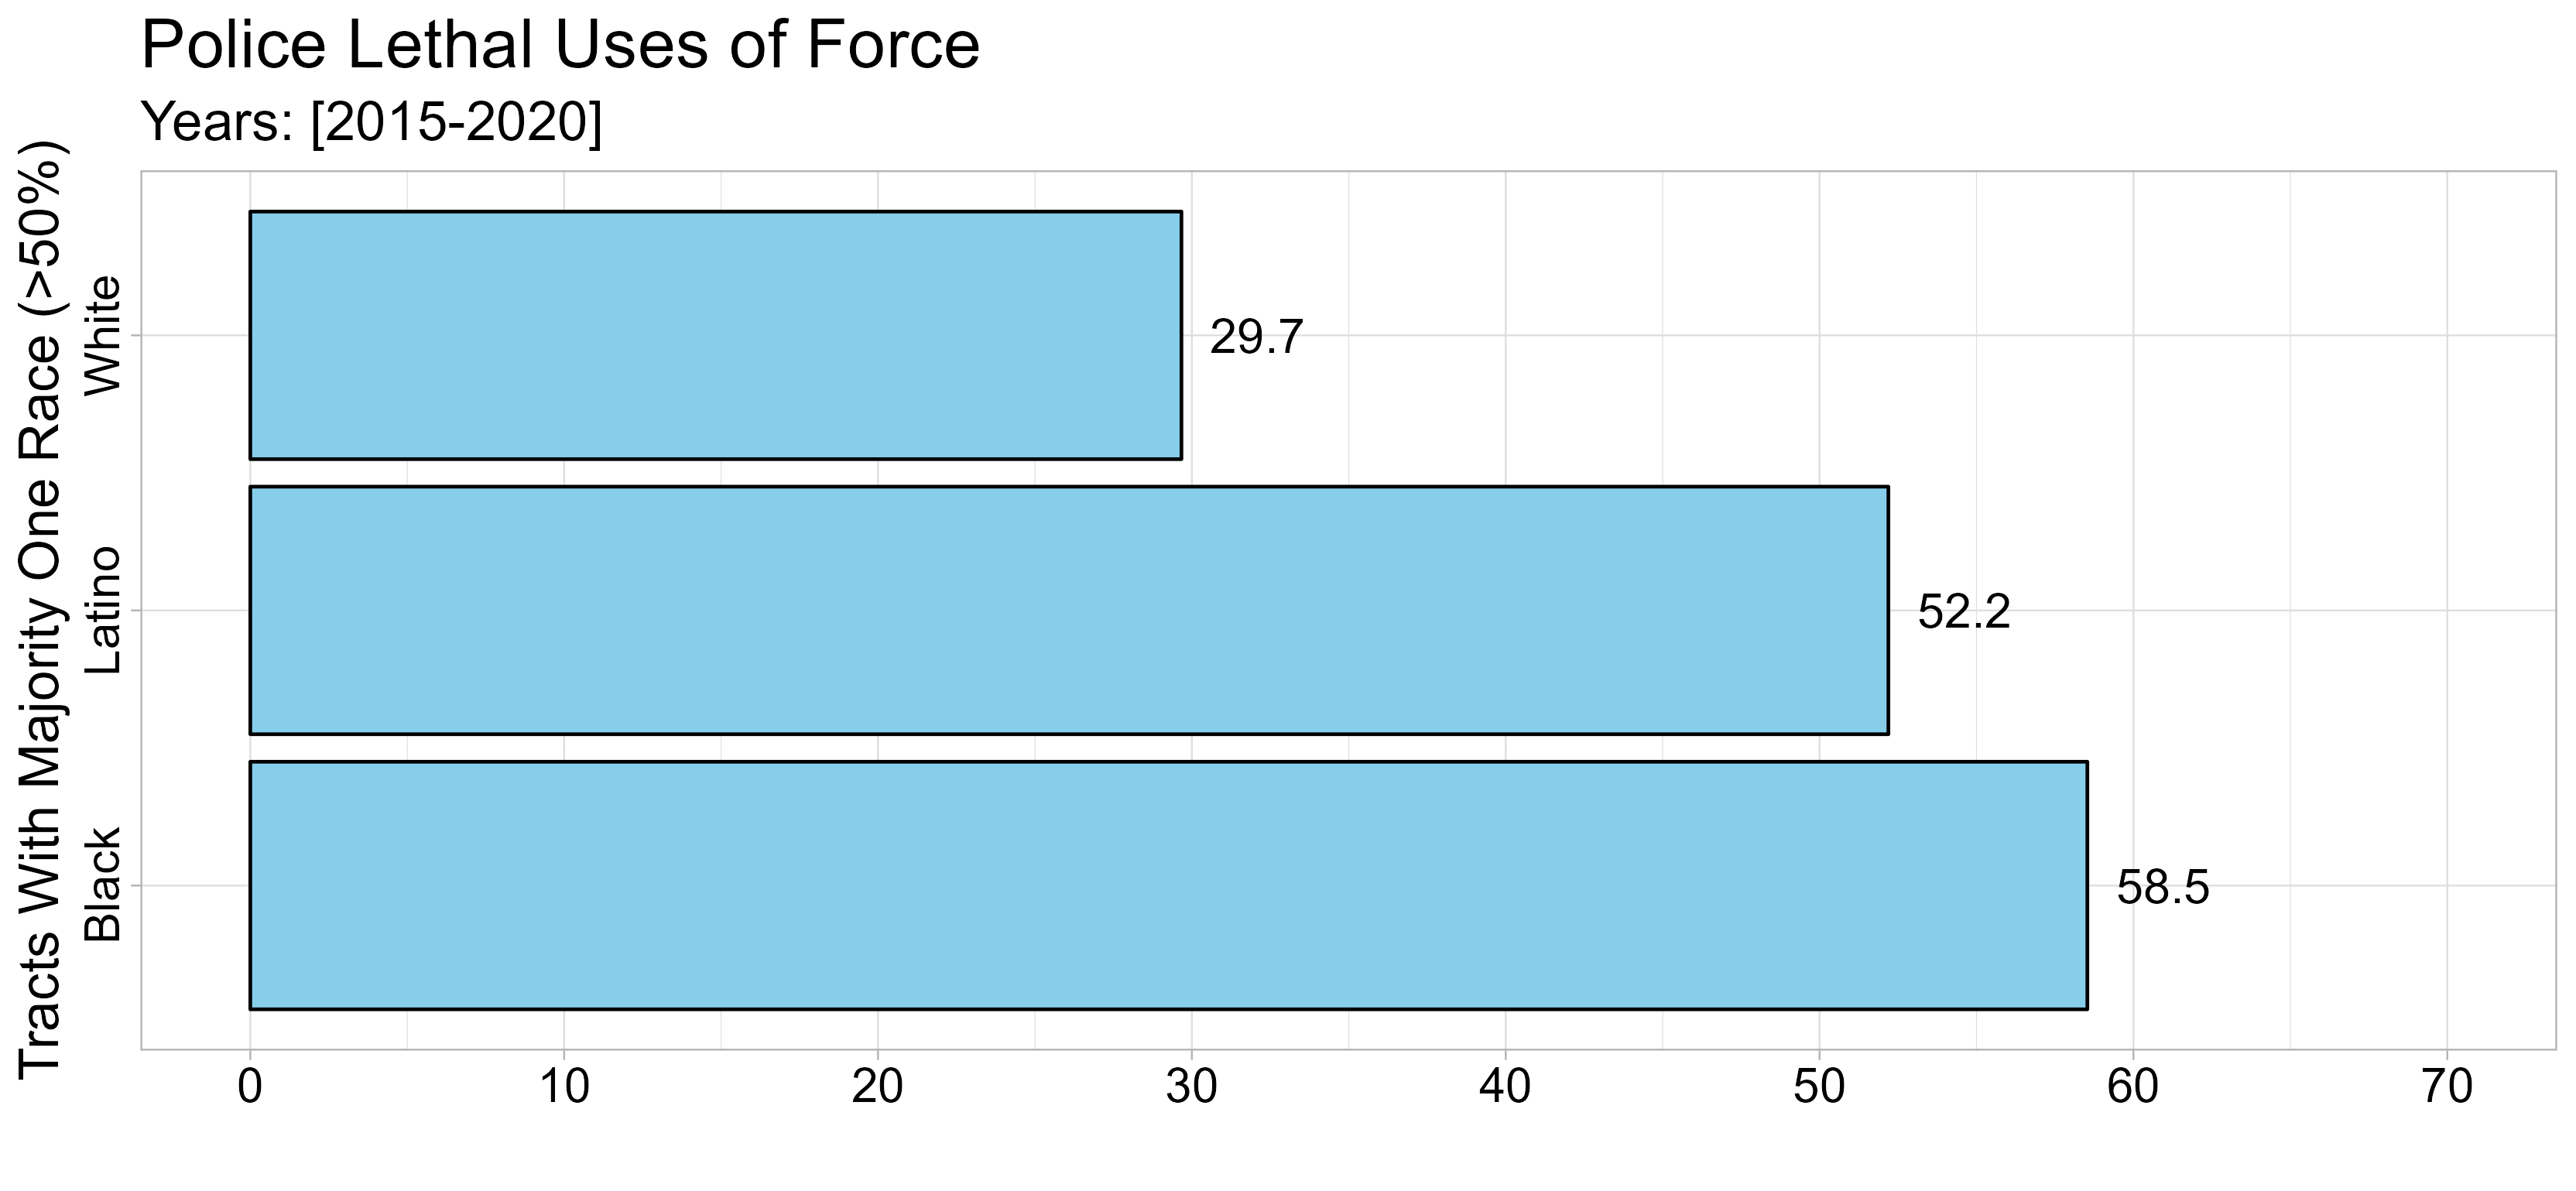
\includegraphics[width=\linewidth]{images/majority_race_only_ind}
  \captionsetup{justification=centering, margin=2cm}
  \caption[Rates by Race and Ethnicity]{Rates by Race and Ethnicity}
  \label{fig:race_ethnicity}
\end{figure}

\noindent{}than majority-white neighborhoods (\autoref{fig:race_ethnicity}).

One possible explanation for the racial disparities is that blacks and Latinos are policed heavily, regardless of how well-off the tract is. A good amount of literature would seem to support this. Many studies have found discriminatory practices within police departments, and there have been many documented incidents of black professionals being harassed by law enforcement, often for rather arbitrary violations. From that perspective, discriminatory practices may largely account for the racial disparities that affect black Americans regardless of their class position. Another possible explanation for these racial disproportions is that blacks and Latinos also disproportionately live in lower-income neighborhoods that are more heavily policed, for reasons discussed earlier. From this perspective, the racial disparities may largely be a function of class position and the way poor and working-class neighborhoods are policed. Of course, these explanations are not mutually exclusive; racial discrimination probably does play some part in generating these racial disparities, while the way the poor are policed could also contribute to the incidence of LUOF. However, it is worth examining the variation within majority one-race census tracts by household income quintiles to see how much of the disparity disappears once household income is introduced into the analysis.

\subsection{Median Household Income}

The American Community Survey (ACS) provides median household income values for each tract. For this analysis, the US census tracts were classified into quintiles based on the distribution of median household income across all US census tracts. Initial analyses show that median household income has a strong relationship with the rate of LUOF (\autoref{fig:income_quintile}). Indeed, LUOFs occur with the highest frequency in the lowest-income tracts. The lowest household income quintile tracts experience a rate more than four times that of the highest household income tracts.

\begin{figure}[H]
  \centering % width=\linewidth, height=0.4\textheight
  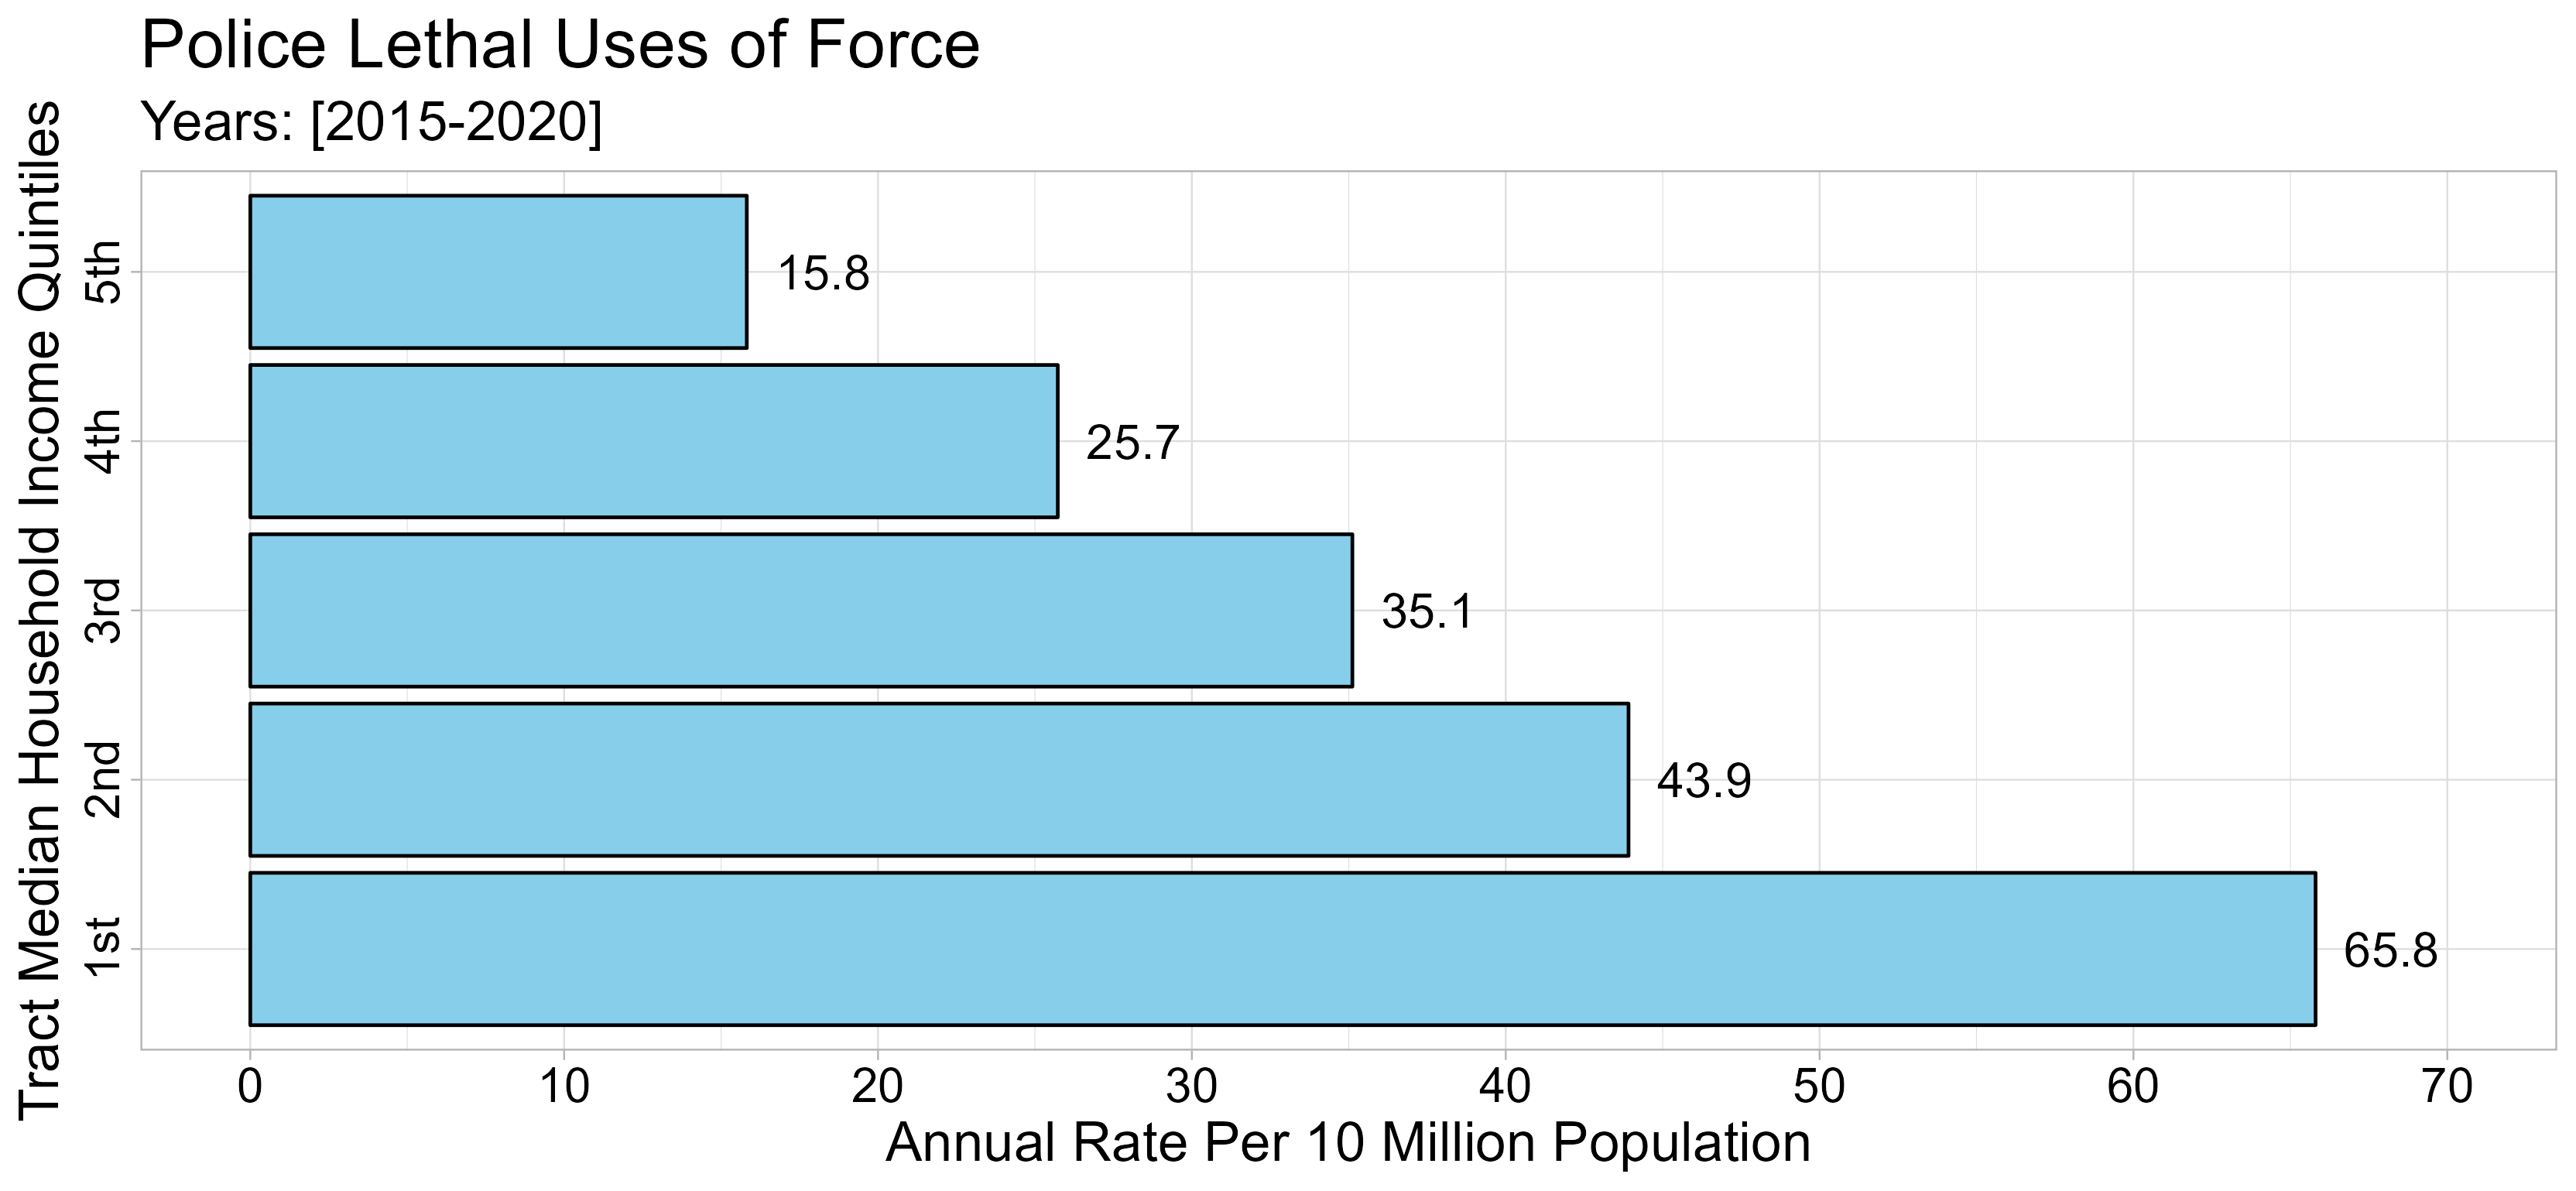
\includegraphics[width=\linewidth]{images/income_quintiles_only_ind}
  \captionsetup{justification=centering, singlelinecheck=false, margin=2cm}
  \caption[Annualized LUOF Rate by Tract Income Quintile]{Annualized LUOF Rate by Tract Income Quintile}
  \label{fig:income_quintile}
\end{figure}

\subsection{Majority One Race}

What, then, does the analysis look like when both race and income are introduced as variables? An initial look at the bar plots by majority-one-race in a census tract and income quintiles offers some useful insights. The plots from earlier are provided again, this time side-by-side on the same scale for easier cross-comparisons. Without looking at their interactions, we can see that the fourth and fifth-quintile census tracts experience a lower rate of LUOFs than any of the racial or ethnic groups. At the same time, both majority-black and majority-Latino census tracts experienced higher rates than all income quintiles except the first or lowest income quintile.

\begin{figure}[H]
  \centering % width=\linewidth, height=0.4\textheight
  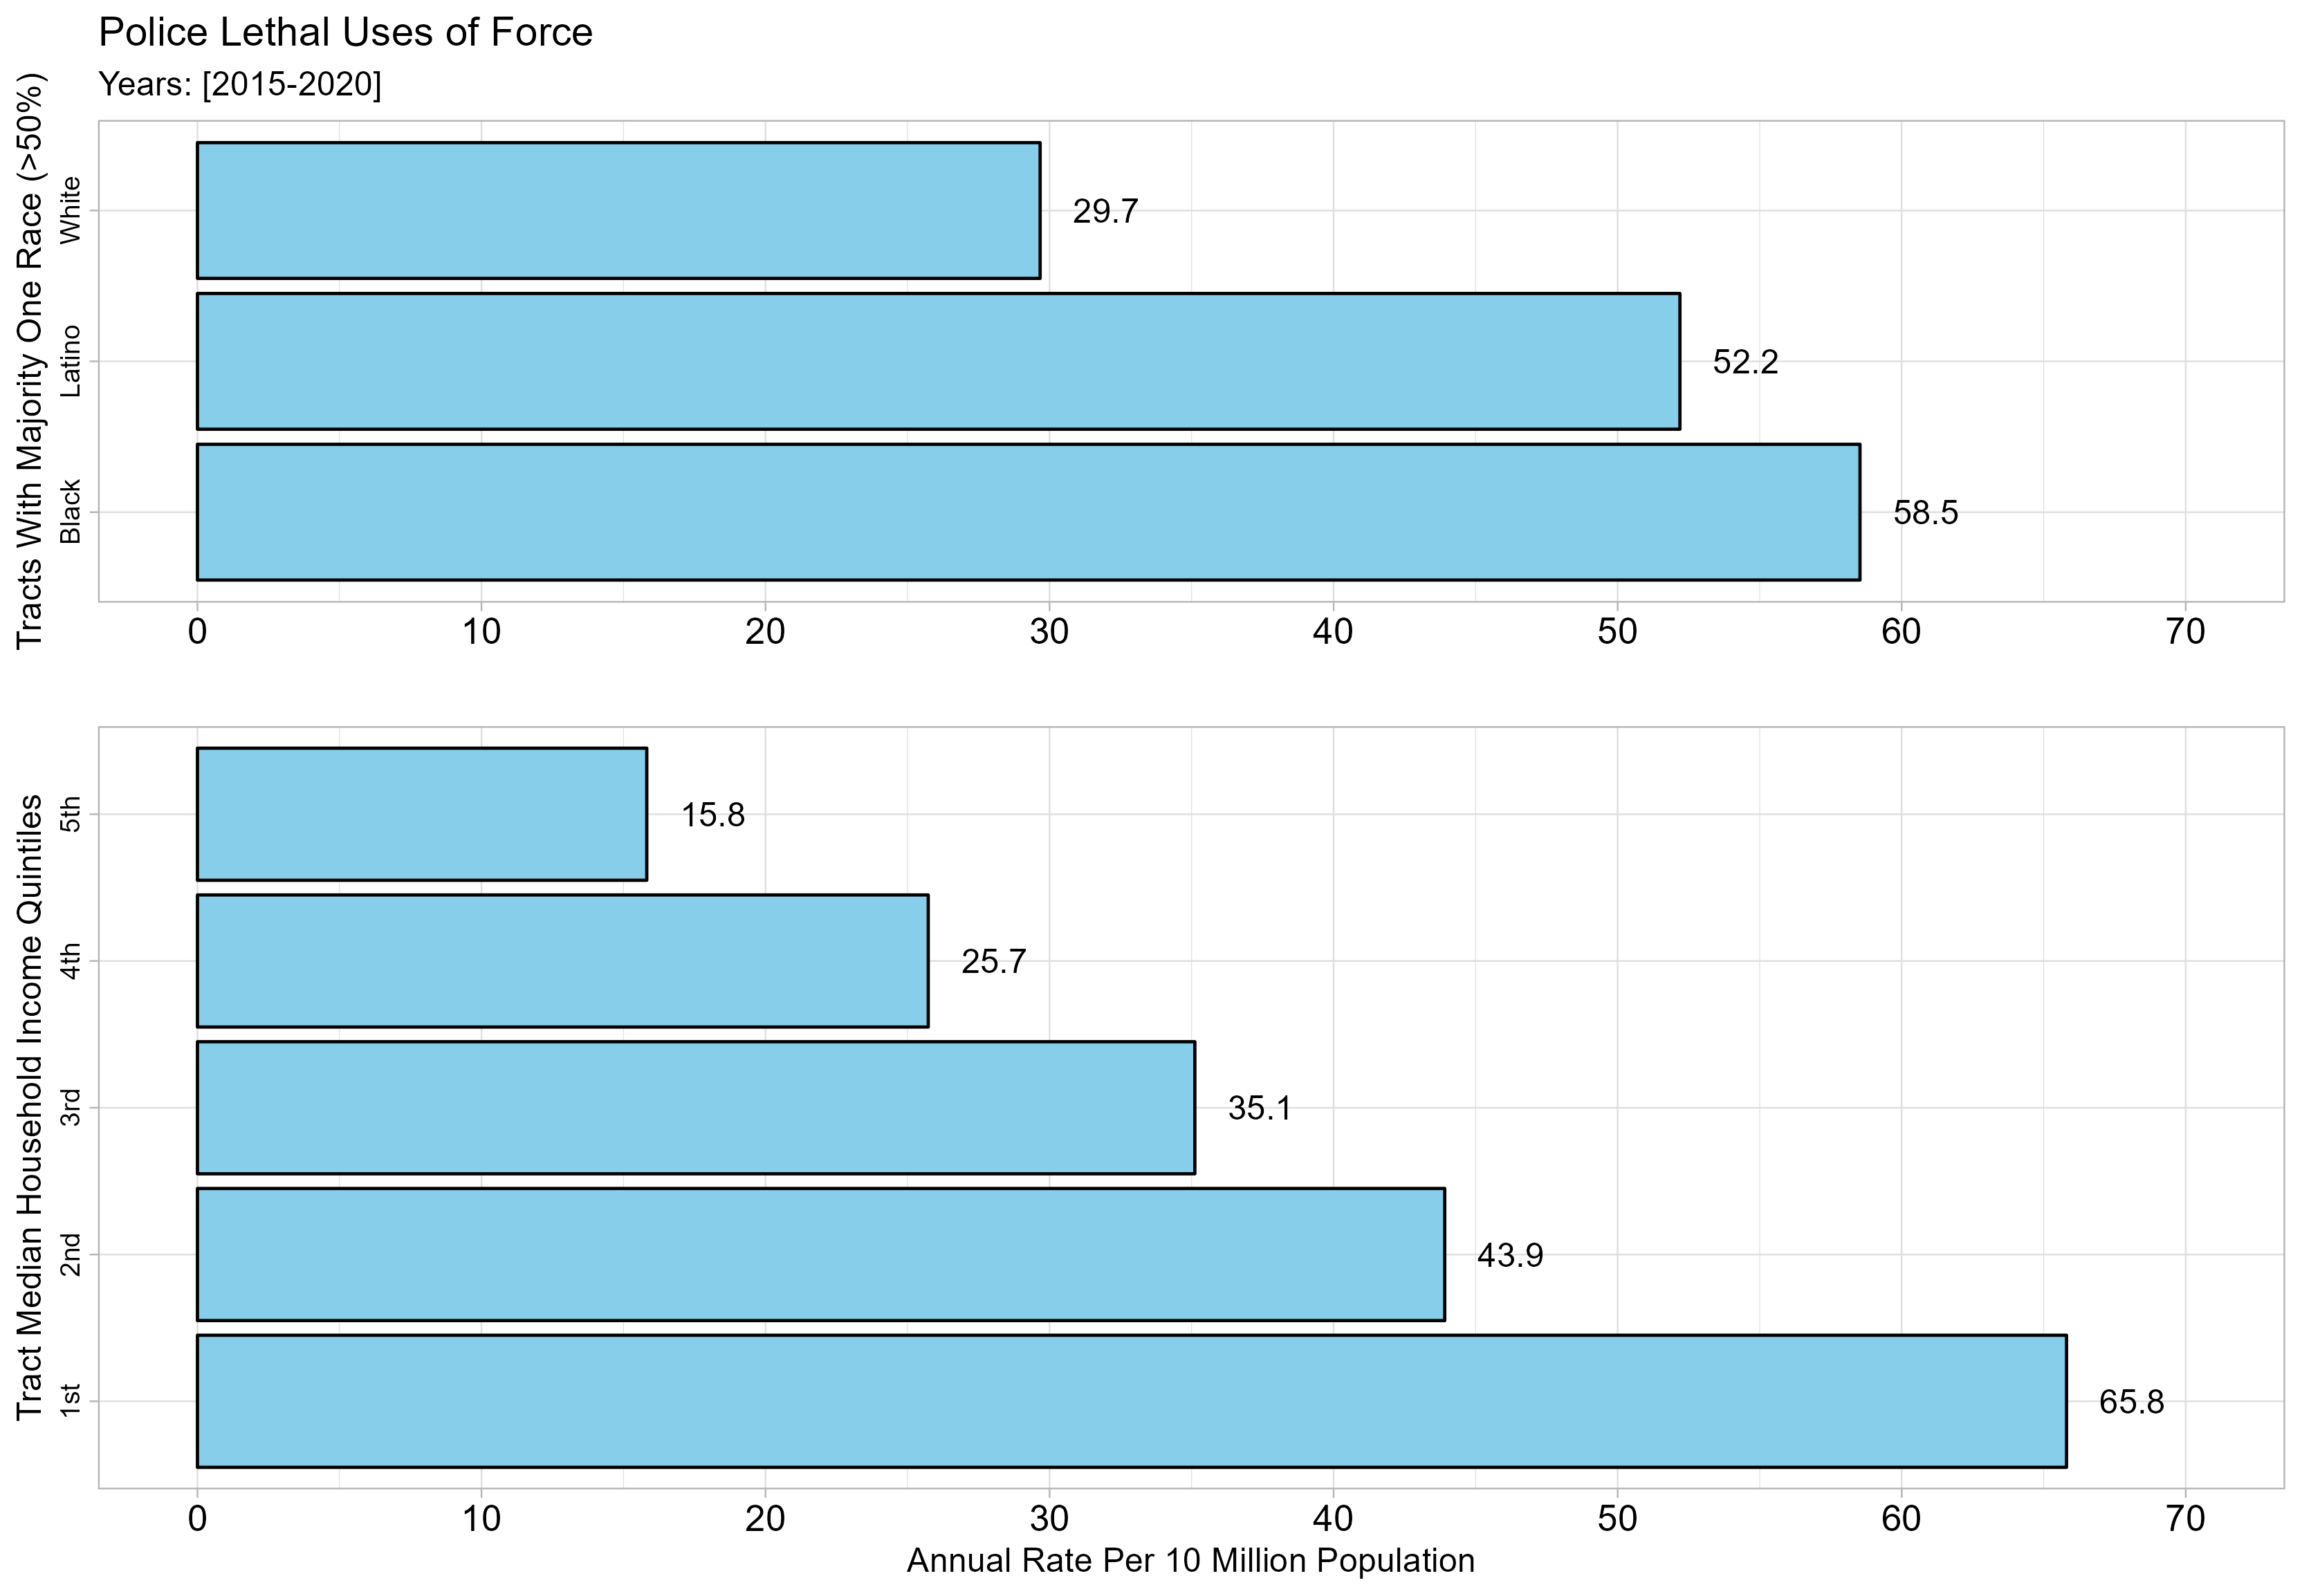
\includegraphics[width=\linewidth]{images/combined}
  \captionsetup{justification=centering, singlelinecheck=false, margin=2cm}
  \caption[Income and Race]{Income and Race}
  \label{fig:combined}
\end{figure}

However, this analysis is inadequate because it does not tell us about the interactions between the variables. In analyzing their interactions, one finds that the general trend of the lowest-income quintiles experiencing the highest rates of LUOFs holds. A bar plot (\autoref{fig:majority_income_interactions}) showing the variation within the racial and ethnic groups indicates that there is substantial variation by income quintile within the racial and ethnic groups. For all racial and ethnic groups, the lowest income quintile had the highest LUOF rate. The difference in the rate between the first and second quintile is substantial for the majority black and Latino census tracts. Majority Hispanic/Latino tracts had the highest rate in the second and third income quintiles. As noted earlier, both the majority-white, and majority-black census tracts experienced the lowest rates of police LUOF in the highest income quintiles.

\begin{figure}[H]
  \centering % width=\linewidth, height=0.4\textheight
  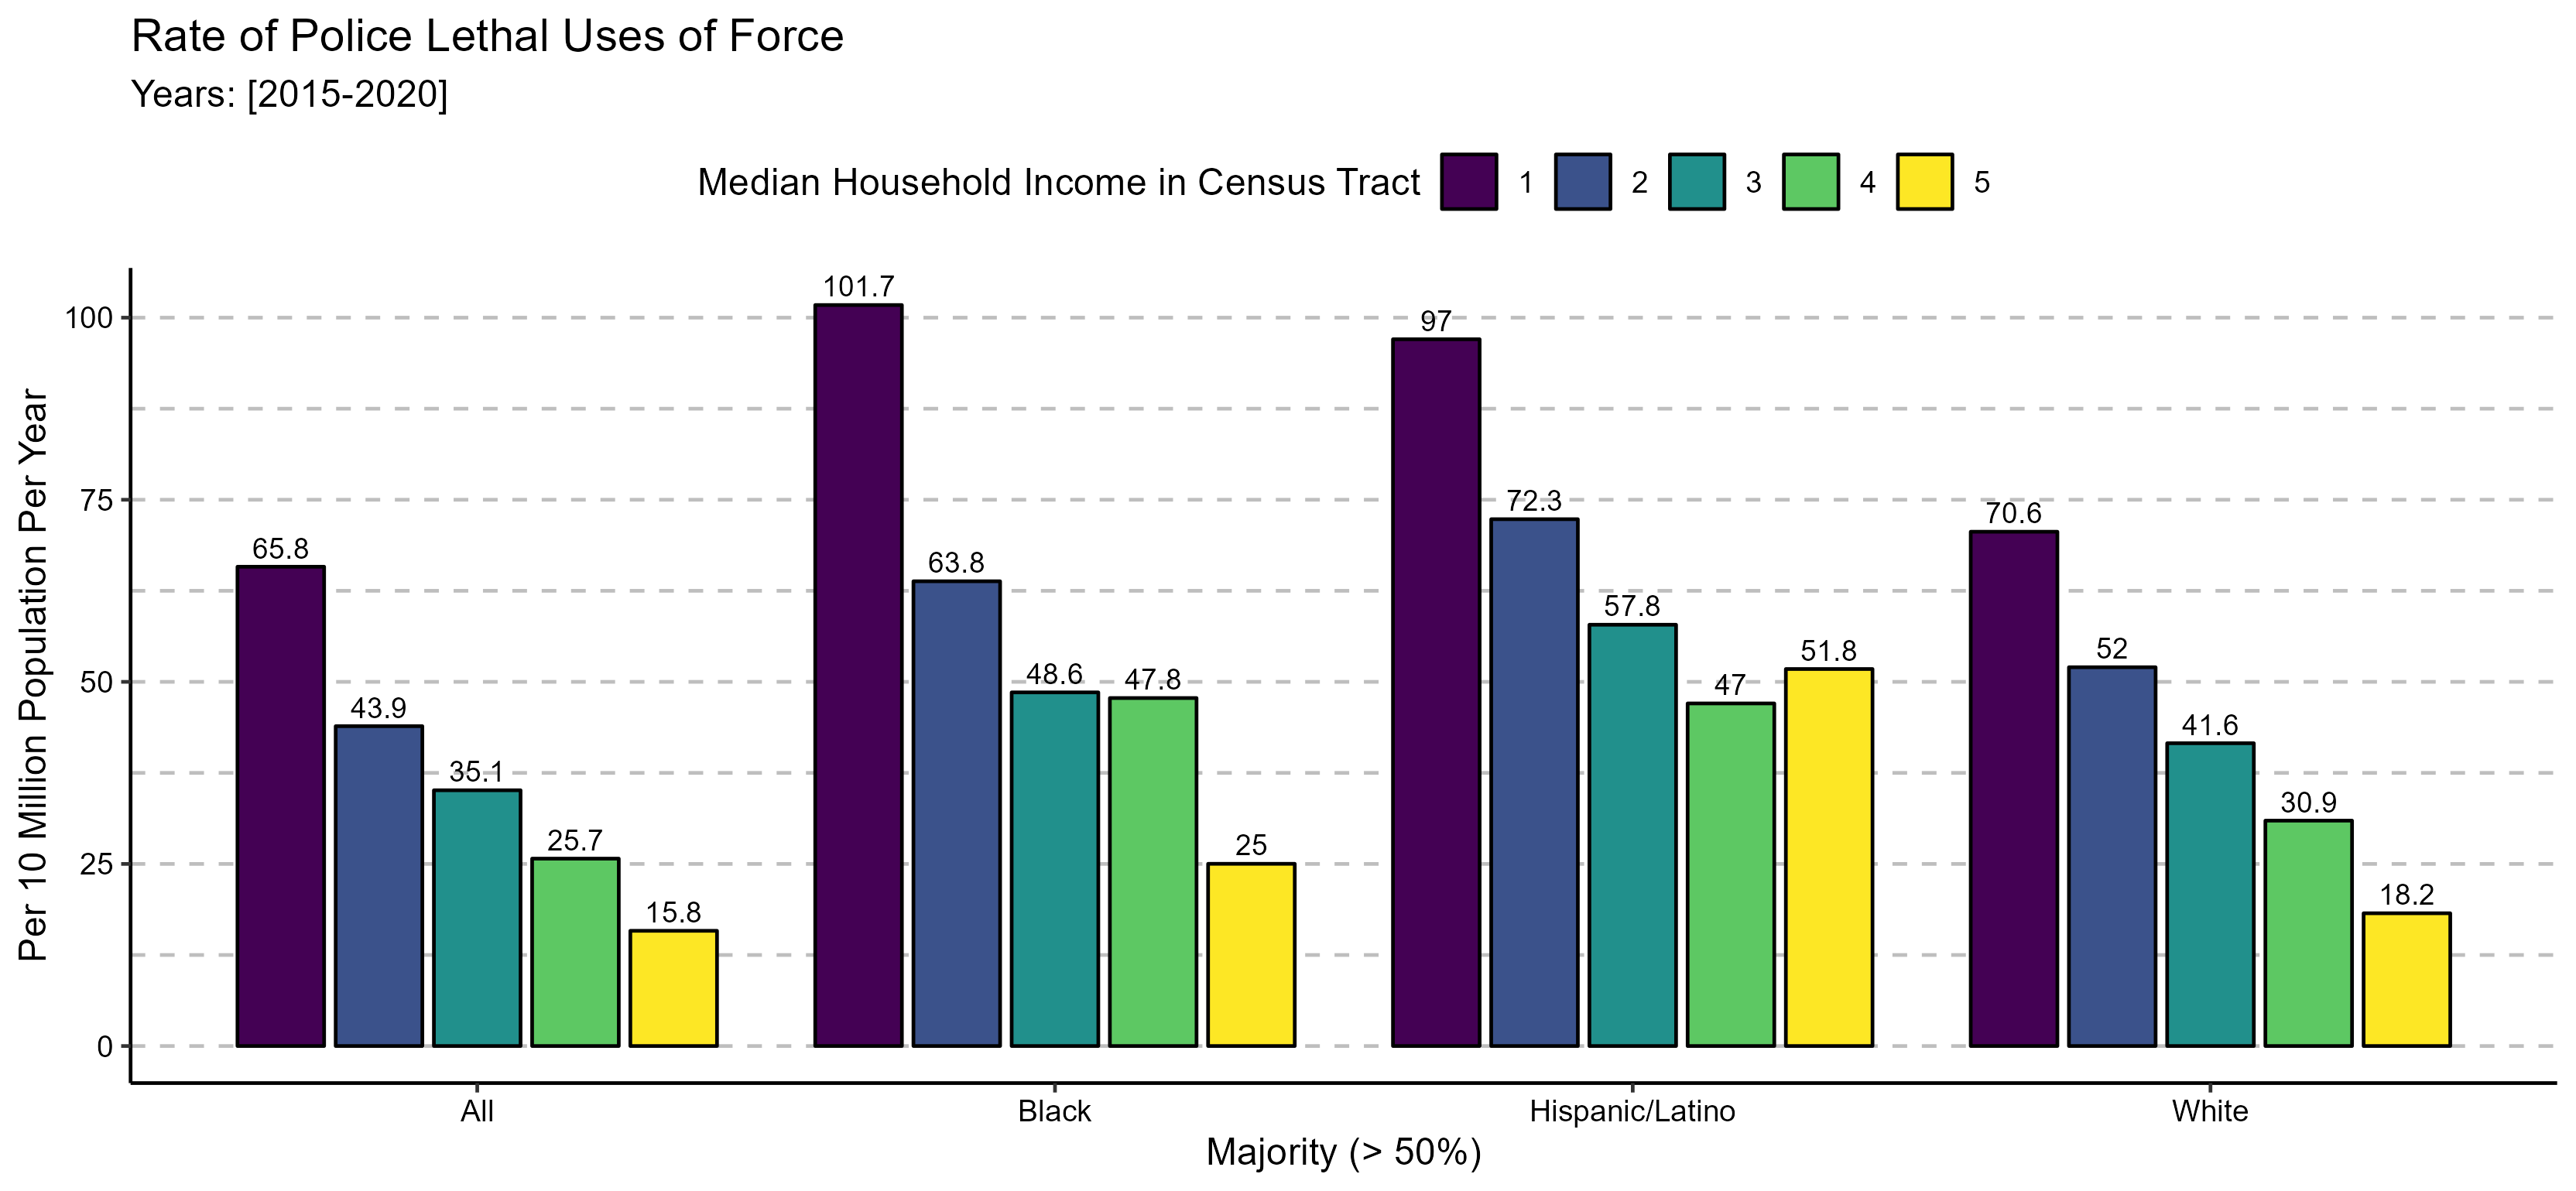
\includegraphics[width=\linewidth]{images/race_only_denom_race}
  \captionsetup{justification=centering, singlelinecheck=false, margin=2cm}
  \caption[Majority Race and Income Interactions]{Majority Race and Income Interactions}
  \label{fig:majority_income_interactions}
\end{figure}

\subsection{Logistic Regression: Income Only}

Because categorizing tracts into majority-one-race tracts sets an arbitrary threshold for inclusion/exclusion from the category, using the proportion of race x living in tract y overcomes this because the proportions are continuous. This allows us to analyze the racial composition of the tract in a more granular way that categorical approaches might flatten out or overlook. For the purposes of the logistic regressions, the median household income is the independent variable, and the dependent variable is a binary variable indicating whether a LUOF occurred between 2015 and 2020 in the census tract. The initial regression included only median household income as a predictor to establish a baseline to understand the effect of income on the probability of being killed by law enforcement. The equation for the regression is:
\begin{equation}
\text{logit}(LUOF_{i})=\beta_{0} + \beta_{1} \times income10k_{i} + \epsilon_{i}
\end{equation}

\noindent{}where \textit{i} is a census tract; \textit{LUOF} is a binary variable indicating whether a LUOF occurred; and \textit{Income}10\textit{k} is the median household income in tens of thousands of dollars.

The regression results show a negative relationship between income and the probability that a tract experienced at least one LUOF during the period (\autoref{tab:income_logit}). A plot of the predicted probabilities indicates a strong curvilinear relationship, with the probability being most pronounced in tracts with incomes of \$50 thousand or less, and the curve flattens somewhat around \$200 thousand. Exponentiating the coefficient results in 0.8758 ($e^{-0.13265}$~=~0.8758), meaning that for every ten thousand dollars in median household income, the odds of a census tract experiencing at least one LUOF declines by 12.42 percent (1~--~0.8758~=~0.1242).

\begin{figure}[H]
  \centering % width=\linewidth, height=\textheight
  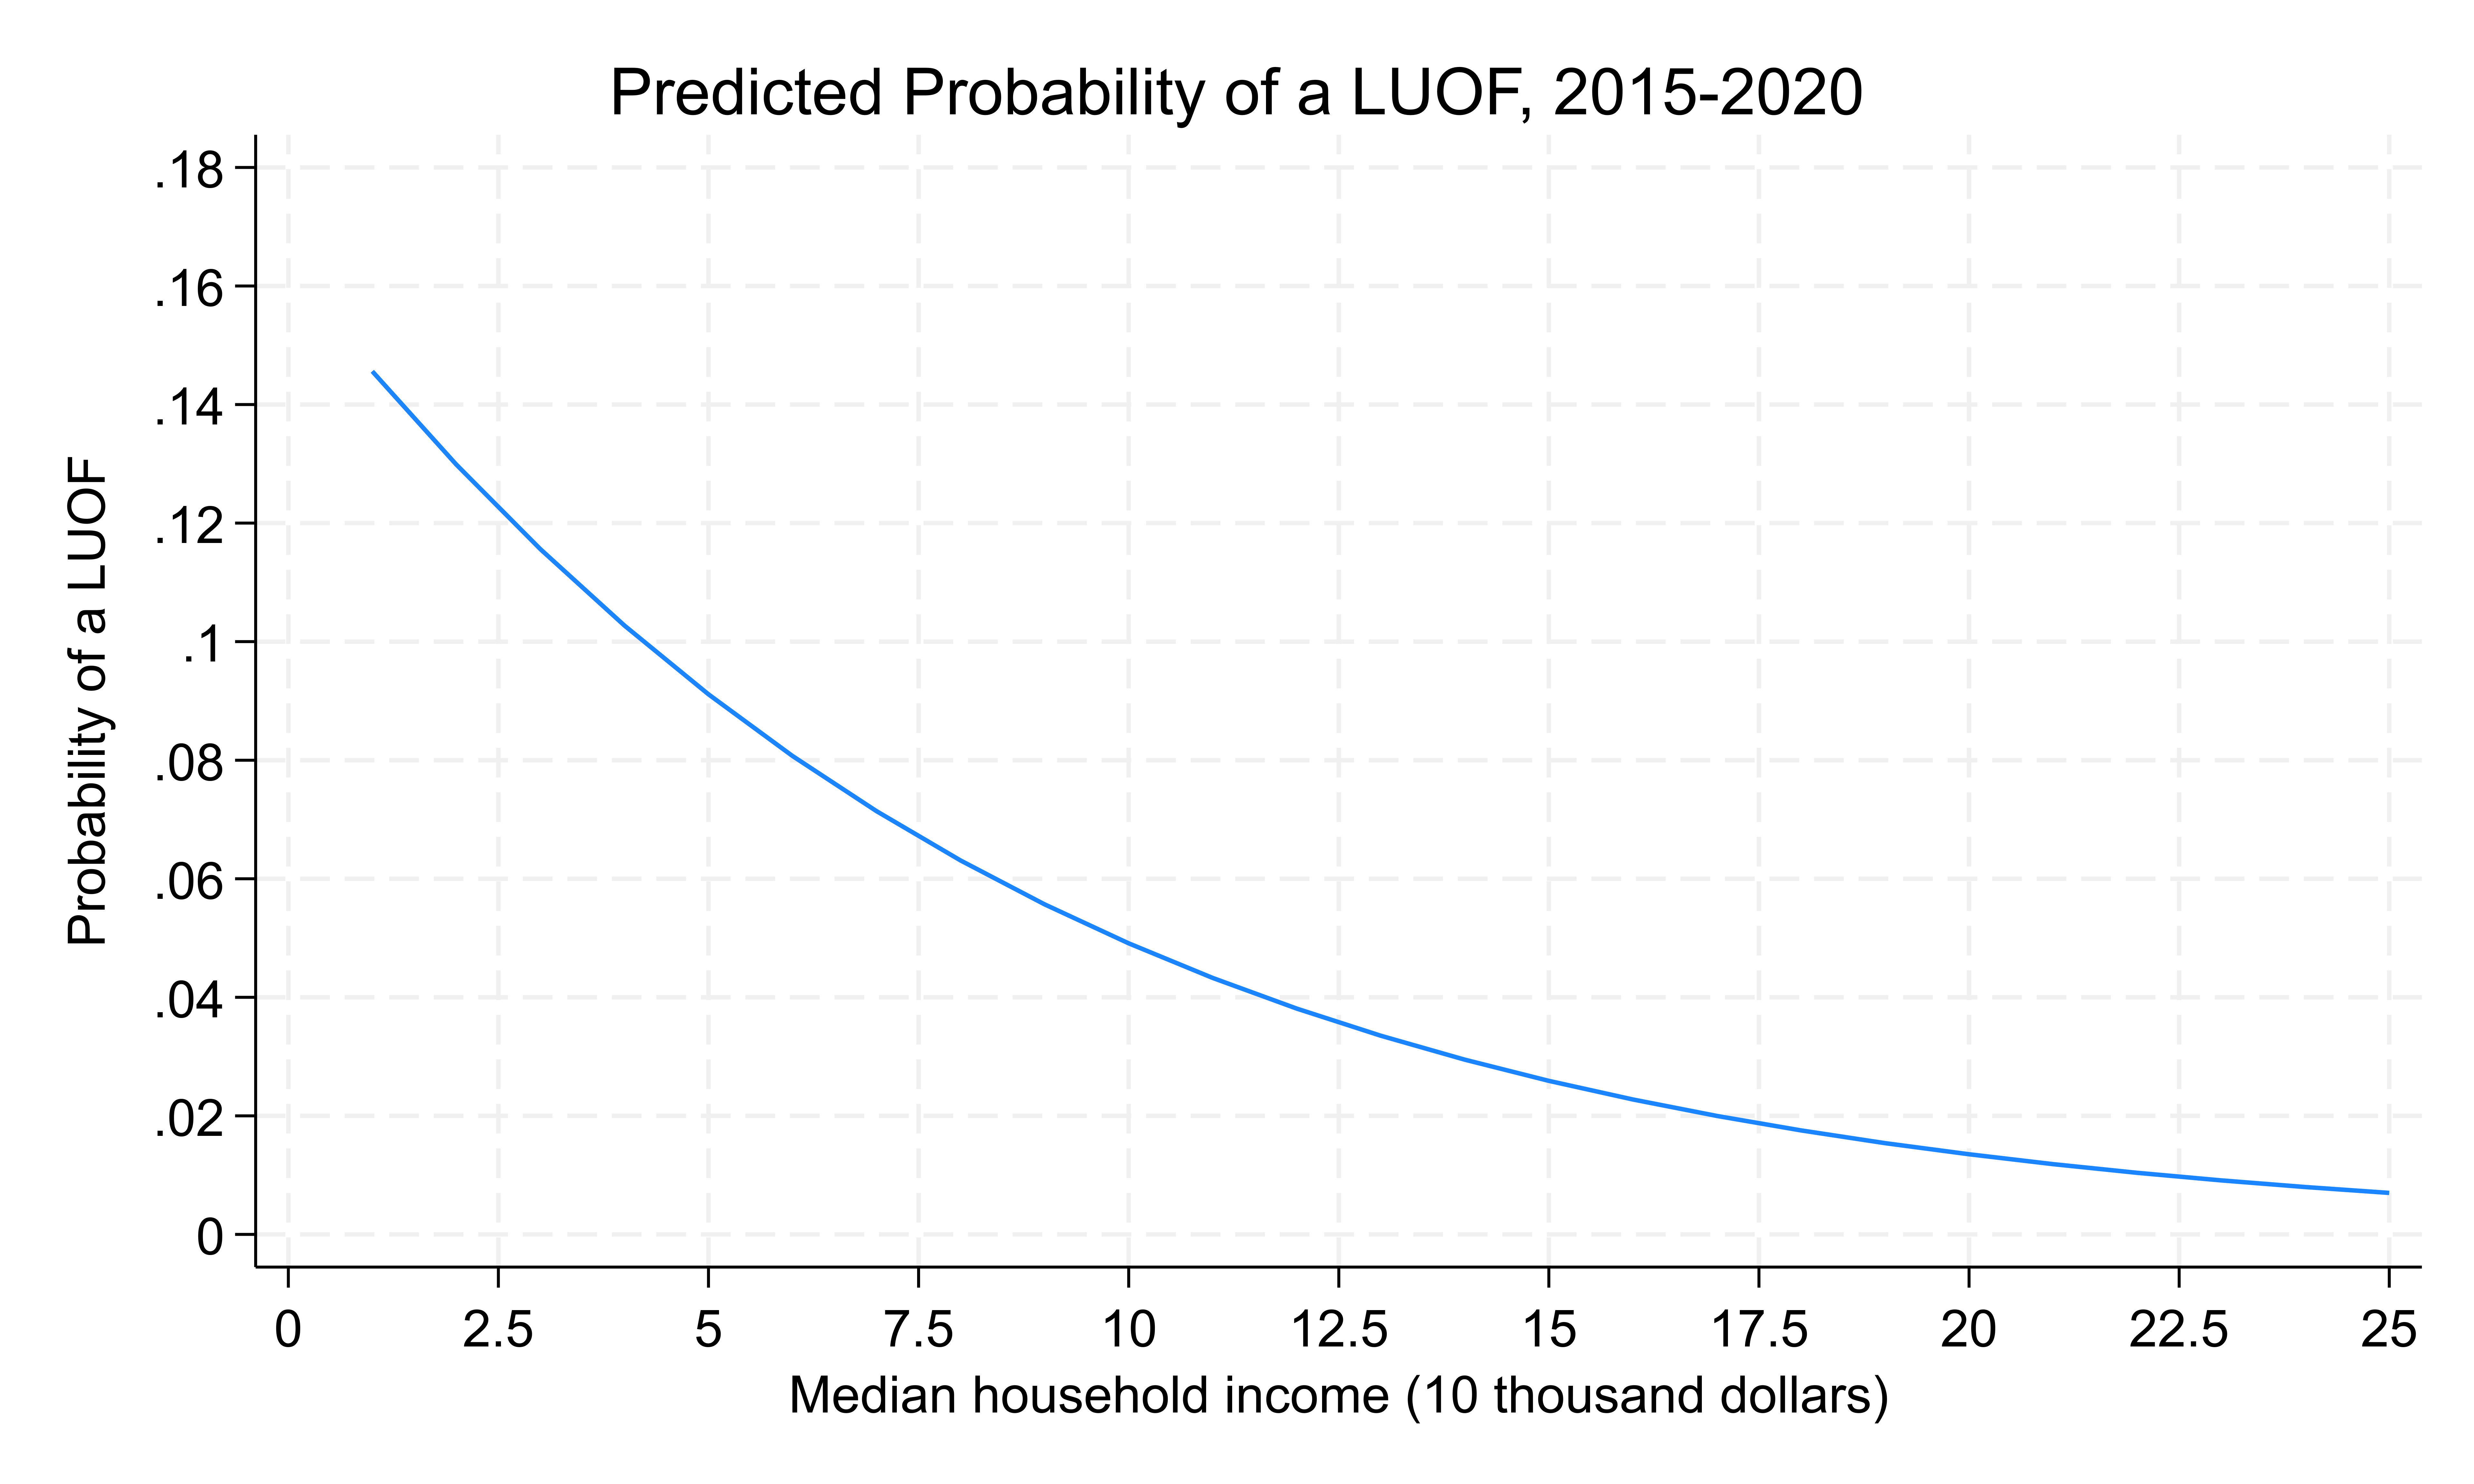
\includegraphics[width=\linewidth]{images/LUOF_logit_income_only}
  \captionsetup{justification=centering, singlelinecheck=false, margin=2cm}
  \caption[Predicted Probability of a LUOF (Income Only)]{Predicted Probability of a LUOF (Income Only).}
  \label{fig:logit_income_plot}
\end{figure}

\begin{table}[ht]
\centering
\begin{tabular}{lcccccc}
\toprule
\textbf{Variable} & \textbf{Coef.} & \textbf{Std. err.} & \textbf{Z-score} & \textbf{P-value} & \textbf{95\% Conf. Int.} \\
\midrule
Income (\$10k) & -0.13265 & 0.0049 & -27.08 & $<$0.0001 & -0.1423, -0.1231 \\
Intercept & -1.636736 & 0.03197 & -51.19 & $<$0.0001 & -1.6994, -1.5741 \\
\bottomrule
\end{tabular}
\caption{Logistic Regression Results for Median Household Income}
\label{tab:income_logit}
\end{table}

\subsection{Bivariate Logistic Regressions: Race/Ethnicity}\

Having established that income is a substantial predictor of whether a LUOF has occurred, logistic regressions were run for each racial/ethnic group to establish to what extent tracts that have a greater proportion of a particular group are more or less likely to have experienced at least one LUOF. The regression equation is:

\begin{equation}
\text{logit}(LUOF_{i})=\beta_{0} + \beta_{1} \times Proportion_{i} + \epsilon_{i}
\end{equation}

\noindent{}where \texttt{i} is a census tract; \texttt{Proportion} is the proportion of the racial or ethnic group living in the \texttt{i}$^\text{th}$ census tract. Three separate regressions were run, one for the proportion black, one for the proportion Hispanic/Latino, and one for the proportion non-white (\autoref{tab:proportions_only}).

\begin{table}[ht]
\centering
\begin{tabular}{lcccccc}
\toprule
\textbf{Model 1} & \textbf{Coef.} & \textbf{Std. err.} & \textbf{Z-score} & \textbf{P-value} & \textbf{95\% Conf. Int.} \\
\midrule
Black Proportion & 0.656 & 0.055 & 11.860 & $<$0.0001 & 0.548, 0.764 \\
Intercept & -2.585 & 0.016 & -164.860 & $<$0.0001 & -2.616, -2.554 \\
\midrule
\textbf{Model 2} & \textbf{Coef.} & \textbf{Std. err.} & \textbf{Z-score} & \textbf{P-value} & \textbf{95\% Conf. Int.} \\
\midrule
Non-White Proportion & 0.9267 & 0.042 & -22.130 & $<$0.0001 & 0.845, 1.009 \\
Intercept & -2.8861 & 0.0234 & -123.4 & $<$0.0001 & -2.9321, -2.840 \\
\midrule
\textbf{Model 3} & \textbf{Coef.} & \textbf{Std. err.} & \textbf{Z-score} & \textbf{P-value} & \textbf{95\% Conf. Int.} \\
\midrule
Latino Proportion & 1.016 & 0.051 & 19.760 & $<$0.0001 & 0.915, 1.117 \\
Intercept & -2.686 & 0.017 & -156.600 & $<$0.0001 & -2.720, -2.653 \\
\bottomrule
\end{tabular}
\caption{Logit Tables: Racial Proportions}
\label{tab:proportions_only}
\end{table}

\begin{figure}[H]
  \centering % width=\linewidth, height=\textheight
  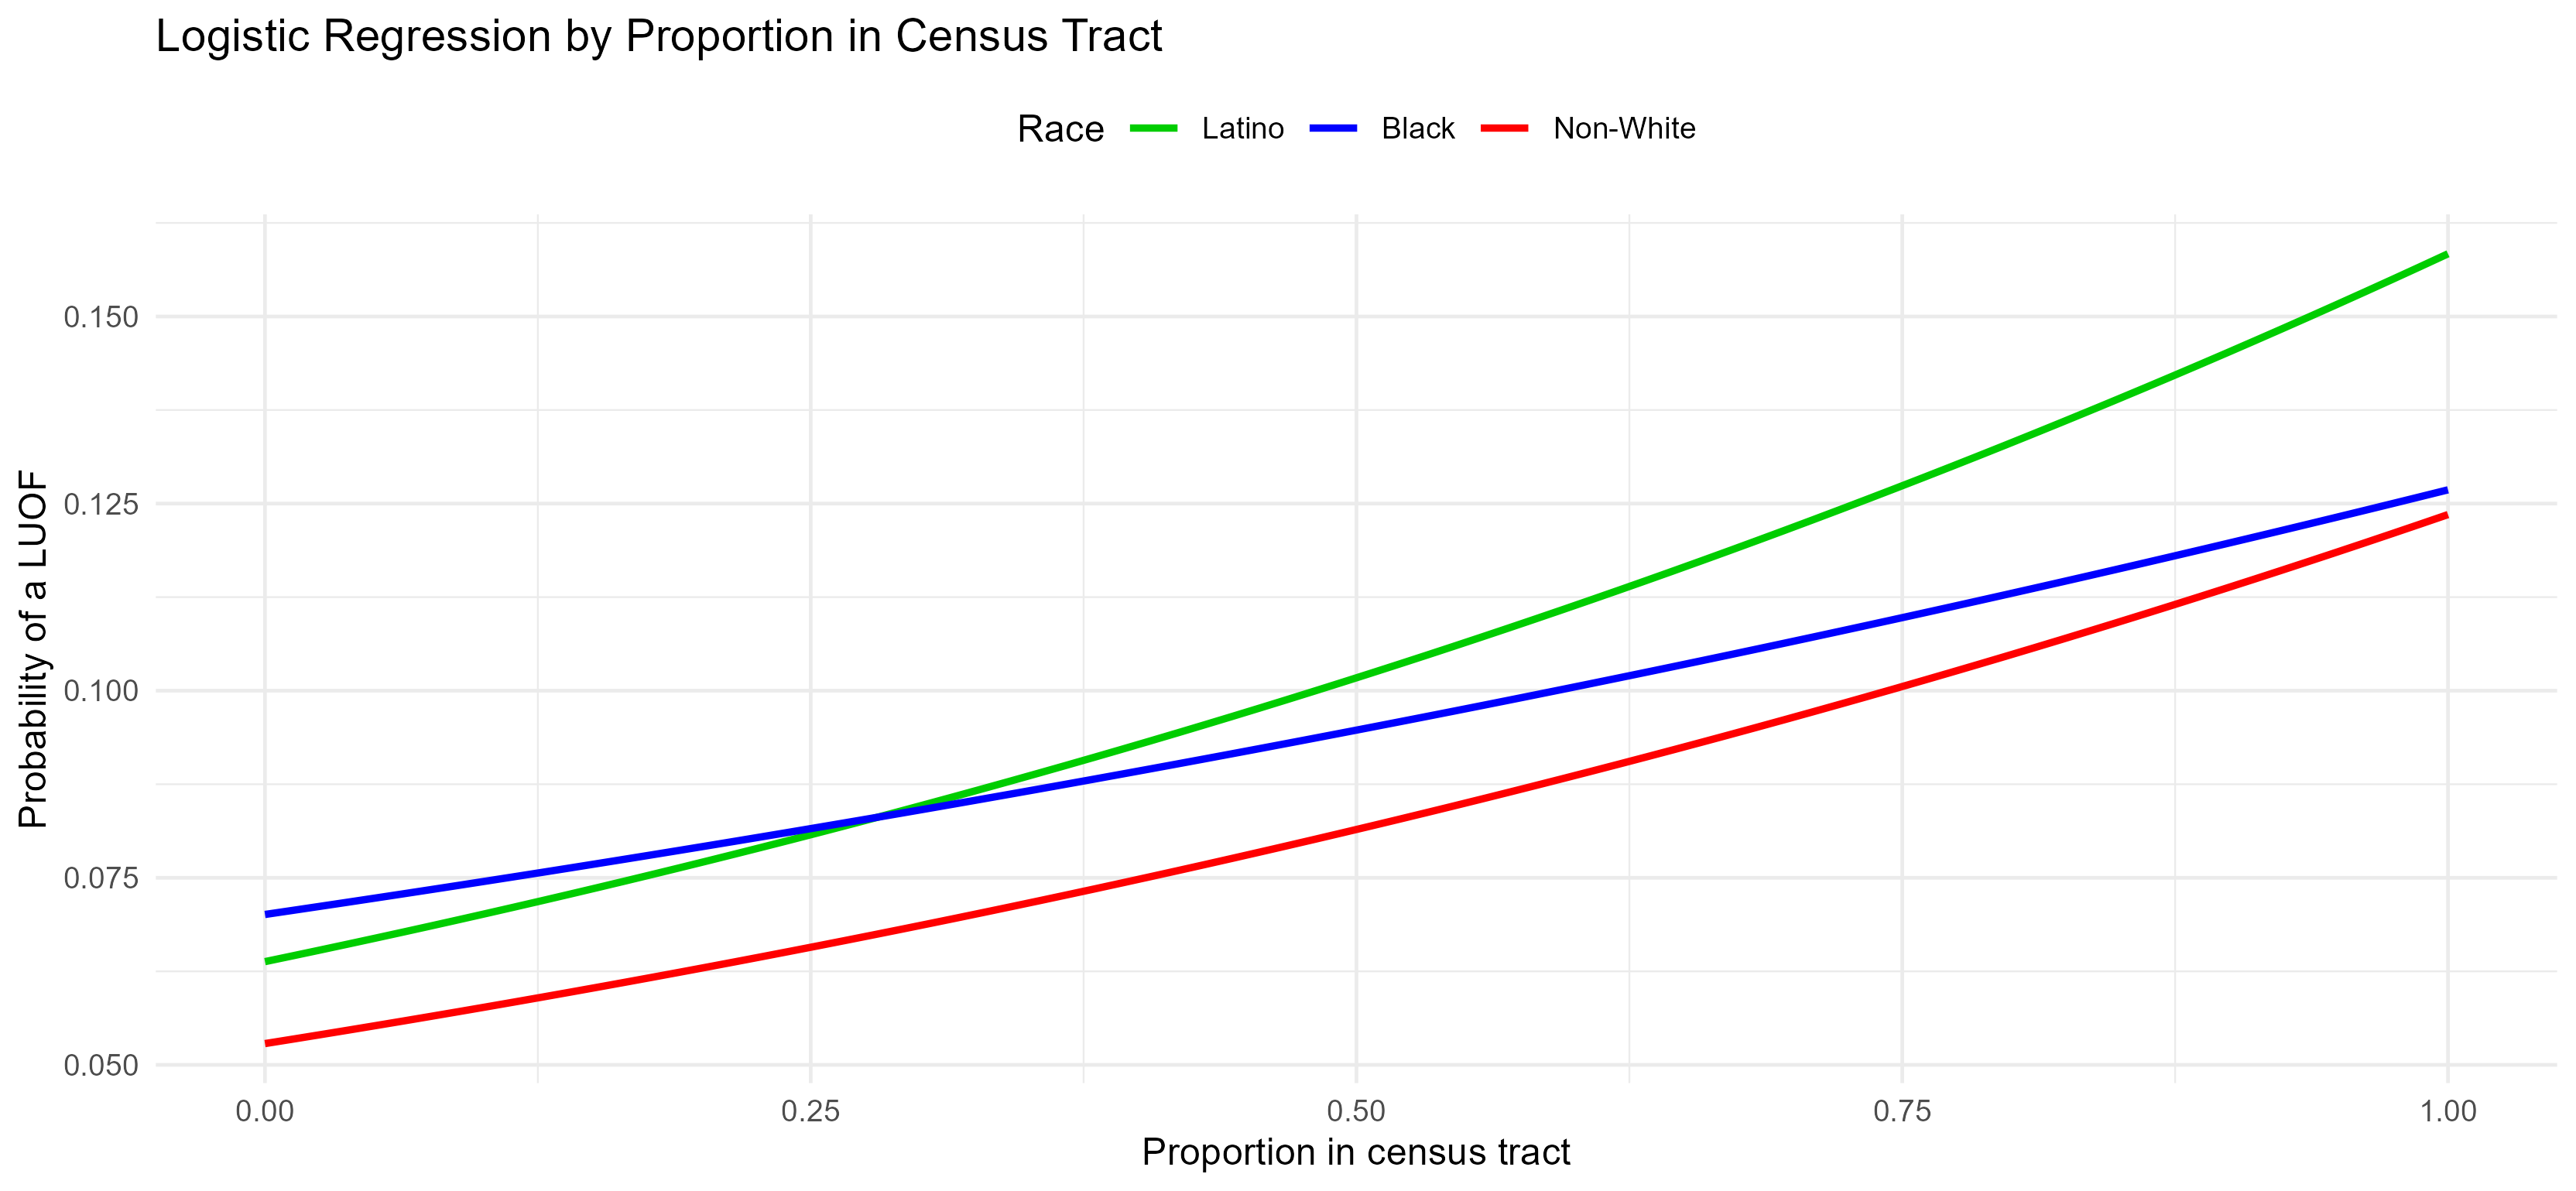
\includegraphics[width=\linewidth]{images/race_proportions_logit}
  \captionsetup{justification=centering, singlelinecheck=false, margin=2cm}
  \caption[Predicted Probability of a LUOF (Race Only)]{Predicted Probability of a LUOF.}
  \label{fig:logit_race_propor}
\end{figure}

\autoref{fig:logit_race_propor} shows that tracts with a greater proportion of blacks and Hispanics/Latinos have a greater probability of having experienced a \acrfull{luof}. Tracts with a high incidence of Latinos have a higher probability of experiencing a \acrshort{luof} than the tracts with the highest incidence of black residents. In addition, tracts with larger non-white proportions also have a higher probability of experiencing at least one \acrshort{luof}. The probabilities are nearly identical for tracts that are 100 percent non-white and those that are 100 percent black tracts.

So, both the income and the racial composition of a neighborhood have a relationship with the probability of a LUOF. Next, regressions with both the racial composition and the median household income were run. This helps establish how much of an effect income has on the probability of a fatal encounter based on the proportion of each racial/ethnic group in the census tract. Marginal effects were calculated and plotted (\autoref{fig:ame_race_by_income}) using the following model:

\begin{equation}
logit(LUOF) = \beta_0 + \beta_1 \text{Income10k}_i + \beta_2 \text{Proportion}_i + \beta_3 (\text{Income10k}_i \ast \text{Proportion}_i) + \varepsilon_i
\label{eq:logit_interaction}
\end{equation}

\noindent{}where \texttt{i} is a census tract; \texttt{Income10k} is the median household income in tens of thousands of dollars in the \texttt{i}$^\text{th}$ census tract; and \texttt{Proportion} is the proportion of the racial or ethnic group living in the \texttt{i}$^\text{th}$ census tract. Again, three separate regressions were run, one for each racial/ethnic group.

\autoref{fig:ame_race_by_income} shows that the \gls{ame} of the racial proportion on the probability of a \acrshort{luof} was greatest for Latinos and non-whites in general, especially in the lowest income tracts. Somewhat surprisingly, the lowest income Latino tracts did not experience the greatest \acrshort{ame} from their higher Latino composition; rather, it is the tracts between \$50 thousand and \$100 thousand that experienced the greatest increase in the probability of \acrshort{luof} as the proportion of Latinos increased. Also, in contrast to folk wisdom, the difference in \acrshort{luof} probability between a tract with zero percent black and 100 percent black composition only appeared in the lower-income black census tracts. In other words, high-income tracts with larger proportions of blacks were no more likely to experience at least one \acrshort{luof} than high-income tracts with small proportions of blacks.

\begin{figure}[H]
  \centering
  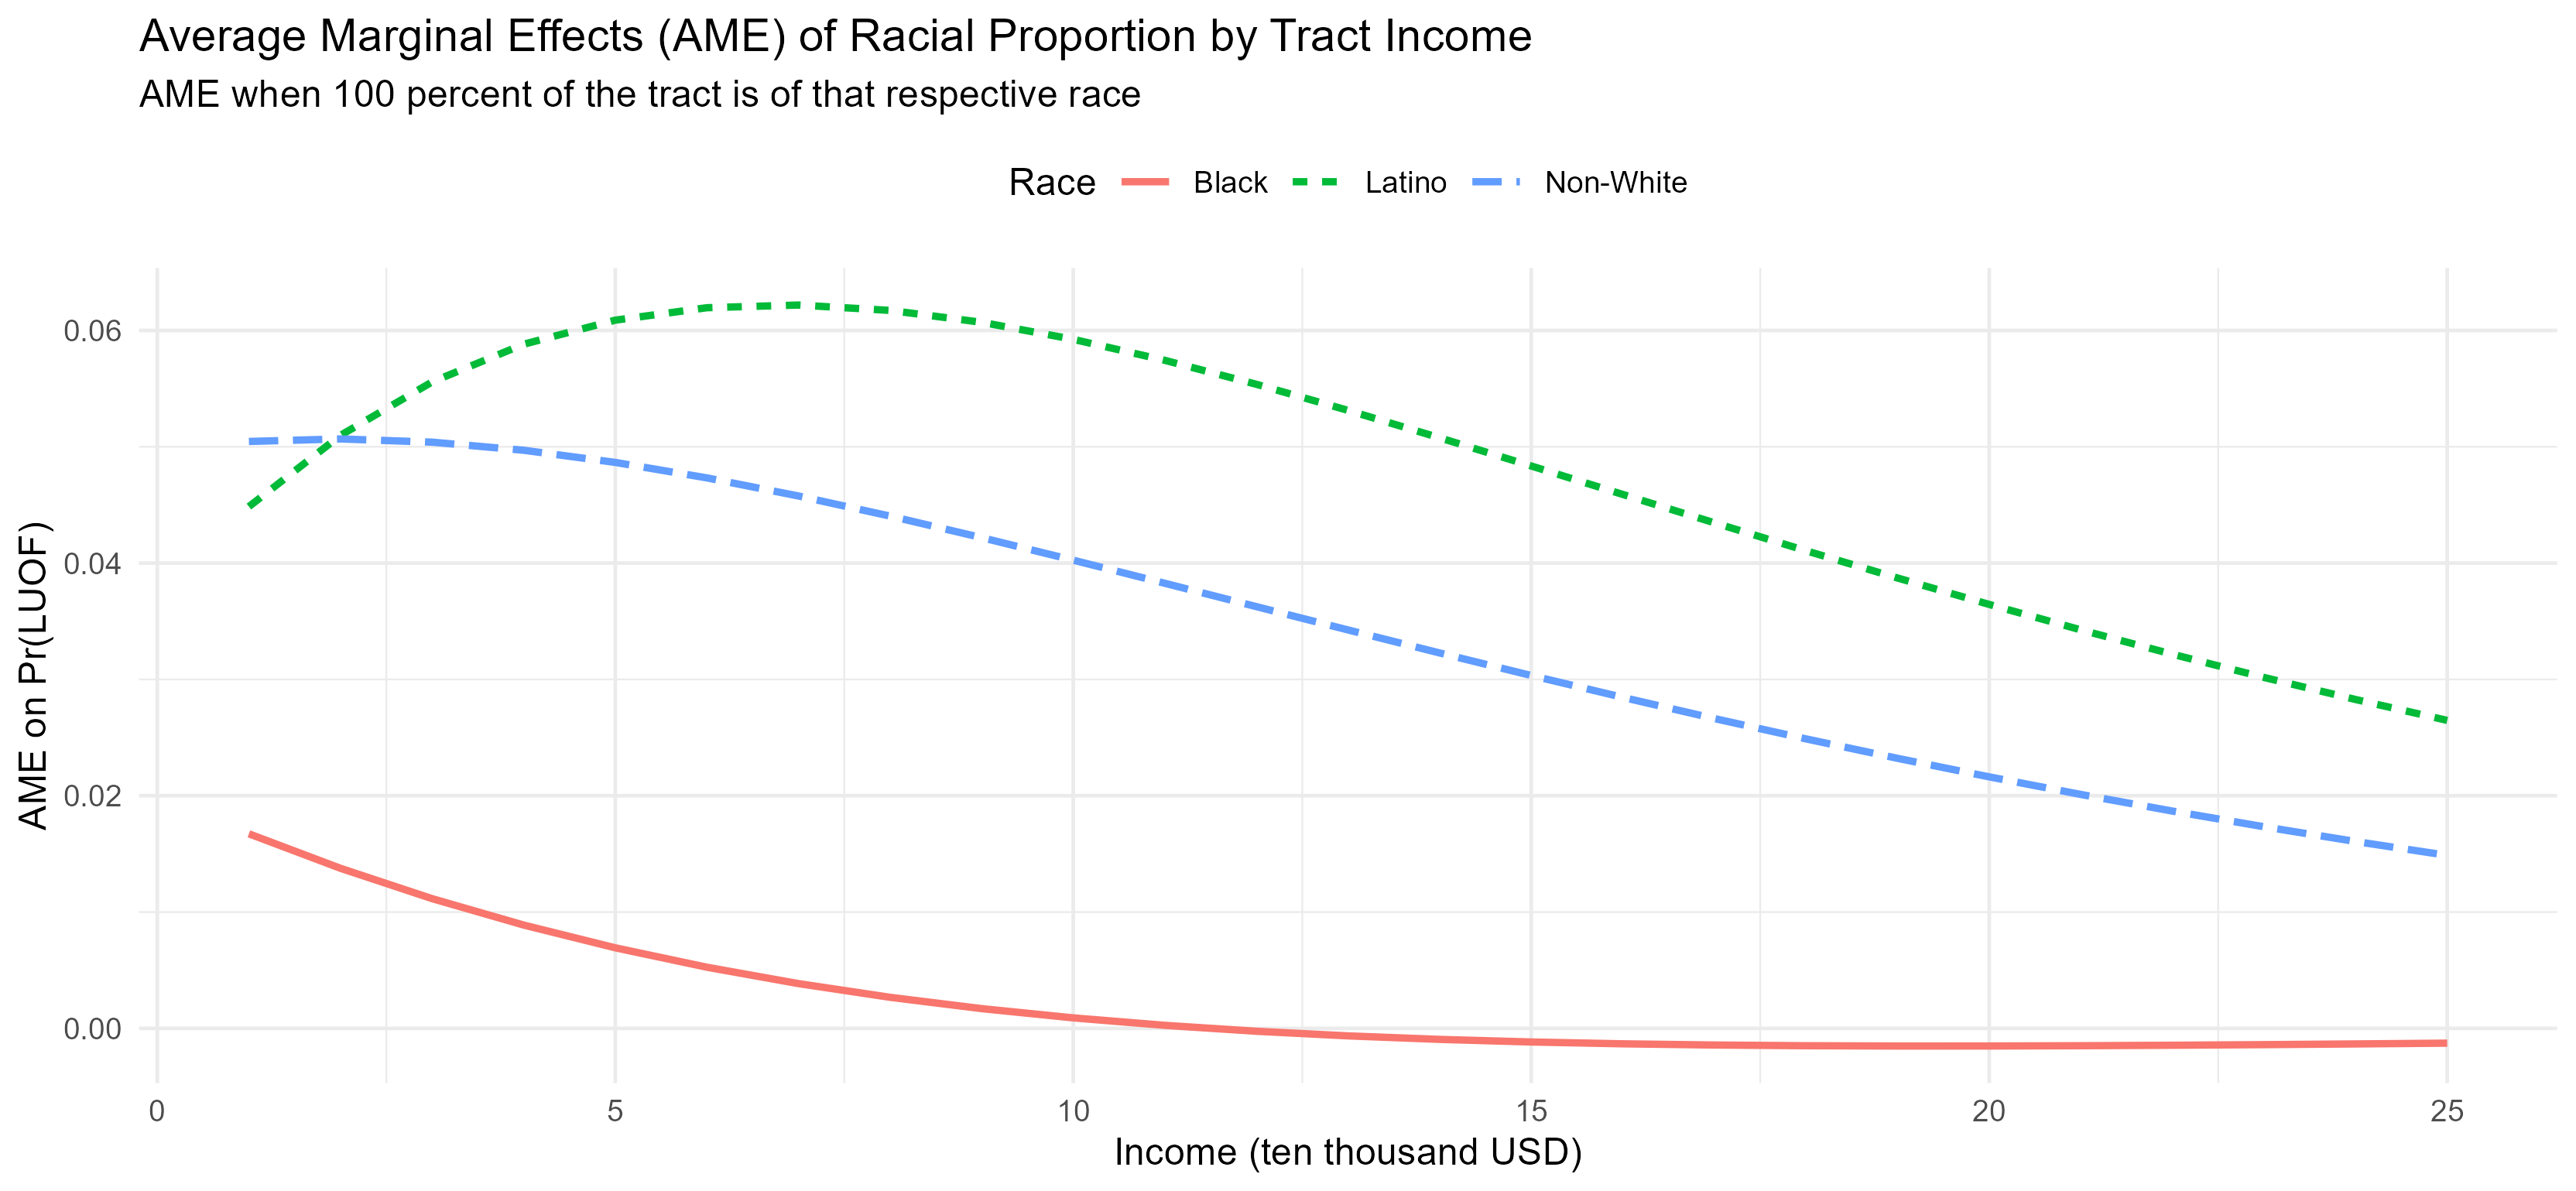
\includegraphics[width=\linewidth]{images/ame_race_by_income}
  \captionsetup{justification=centering, singlelinecheck=false, margin=2cm}
  \caption{Average Marginal Effects of Racial Composition}
  \label{fig:ame_race_by_income}
\end{figure}

\subsection{Race of Victim}\

For robustness, an analysis by race of the victim was also conducted. Using the Fatal Encounters dataset, I constructed a frequency table of the number of LUOFs of victims by race. Contributors to Fatal Encounters imputed a small percentage of these observations ($<$ 9\% imputed). The distribution across racial groups in these six years shows that nearly half of those killed by law enforcement are white; slightly more than 25 percent are black; and approximately 18 percent of those killed by law enforcement are Latino/Hispanic (\autoref{fig:race_proportion_of_total_bar}). There is also a disparity between whites and blacks. Blacks comprise 25 percent of those killed by law enforcement, while their incidence in the broader population is only about 13 percent. On the other hand, whites are killed by law enforcement at a rate slightly less than their incidence in the broader population. At the same time, it is worth a closer look at how the LUOF victims are distributed across tract income quintiles within each racial group.

\begin{figure}[H]
  \centering
  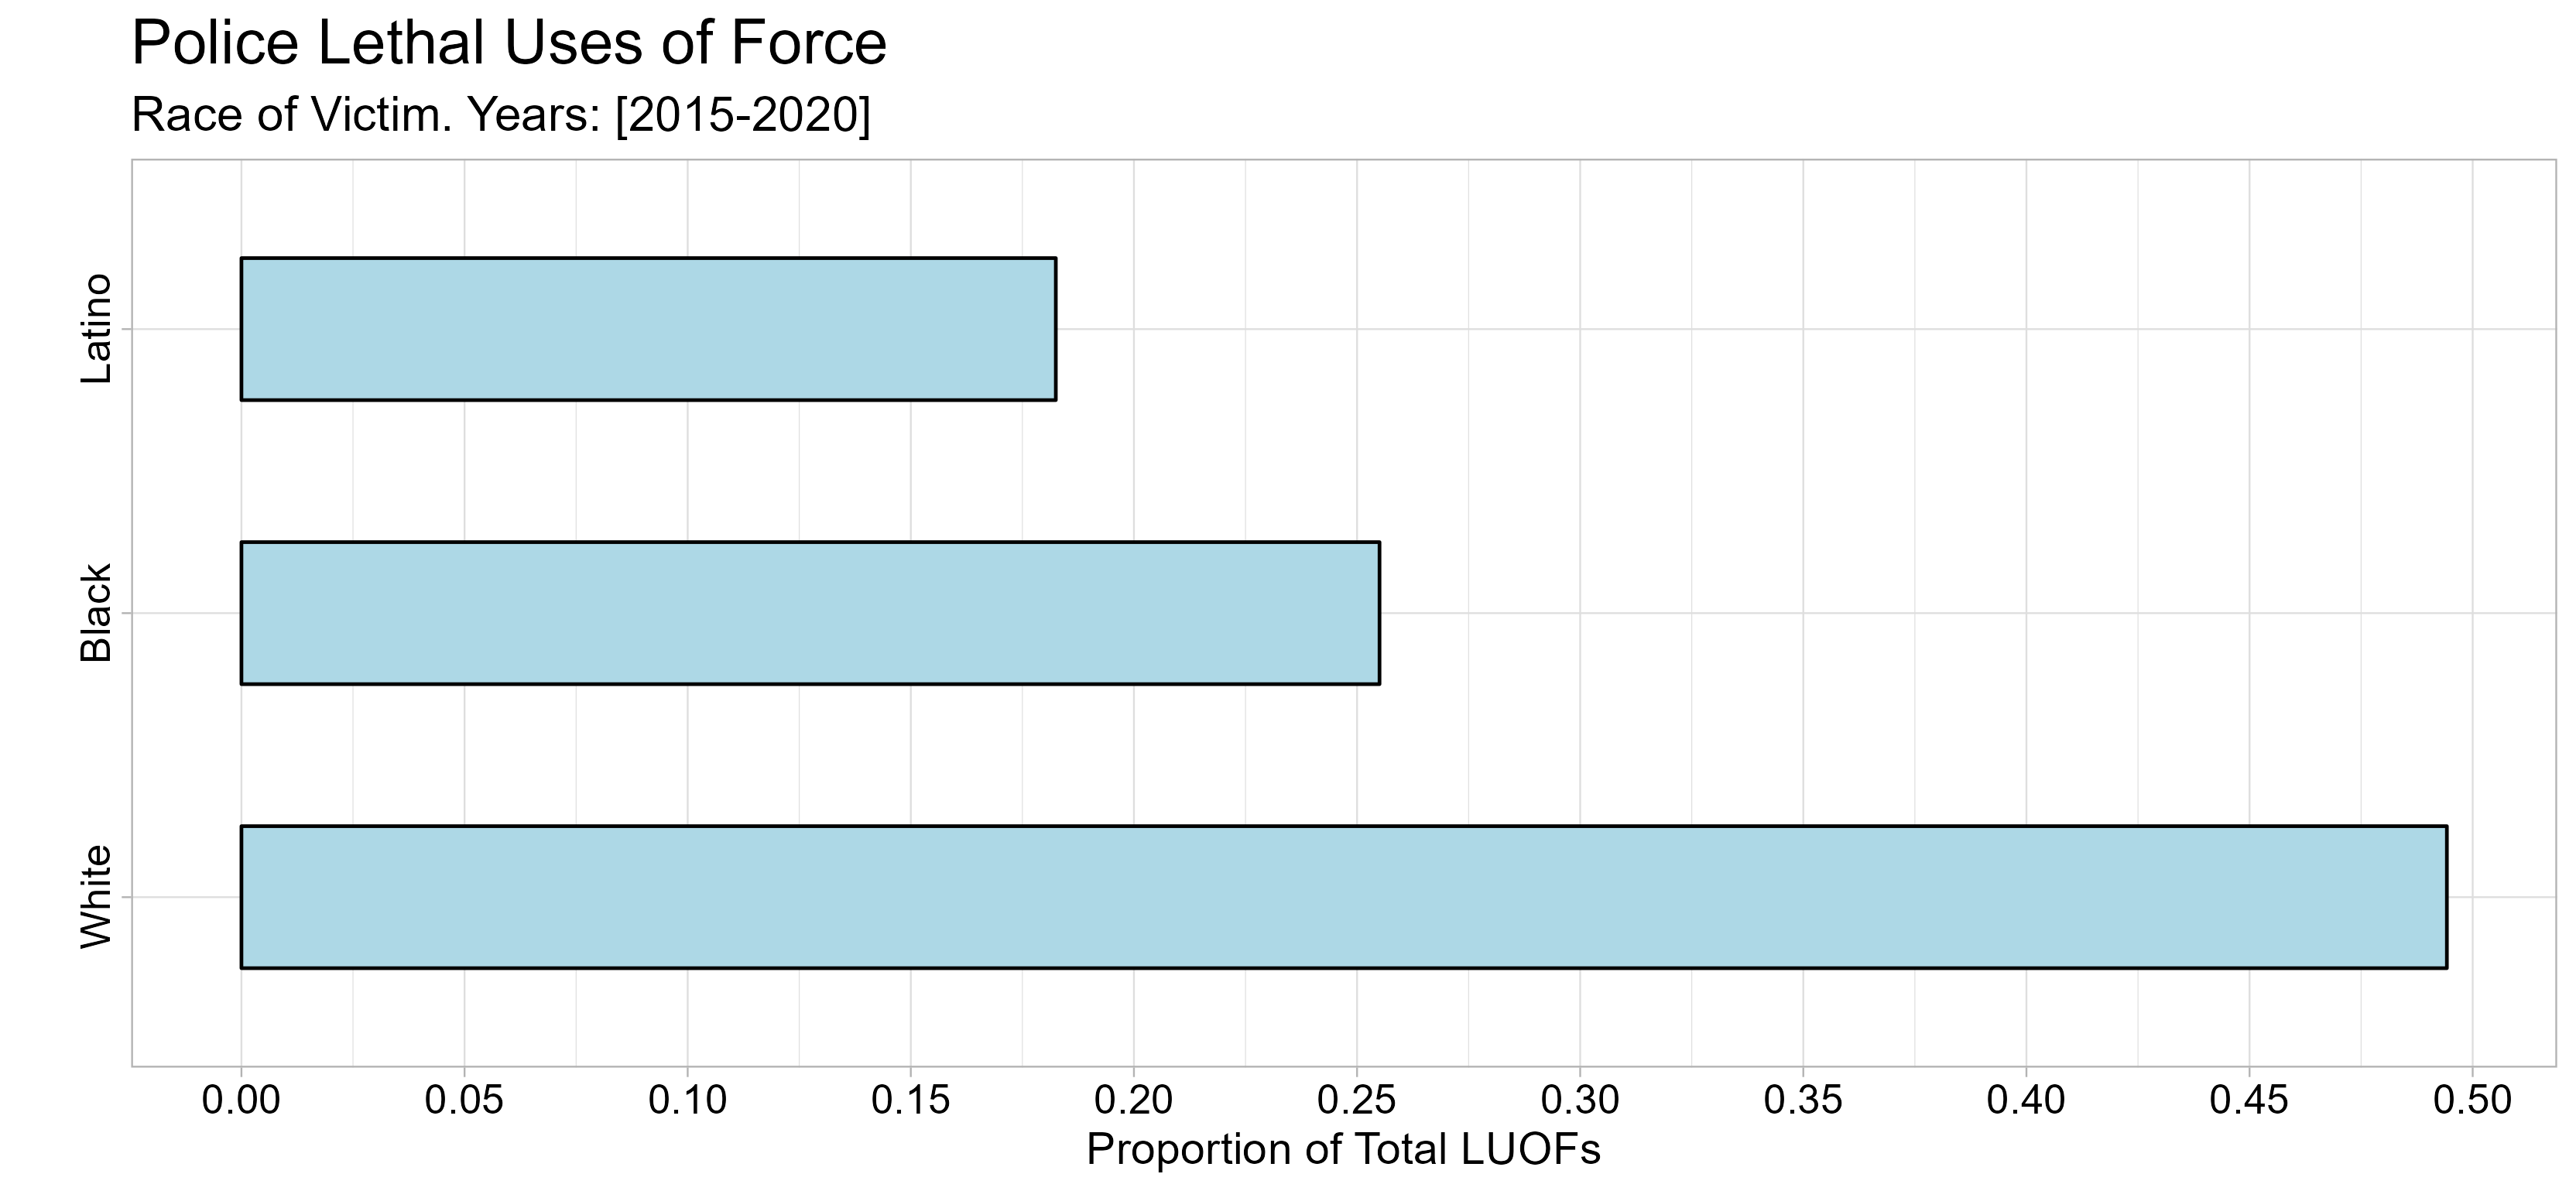
\includegraphics[width=\linewidth]{images/race_proportion_of_total_bar}
  \captionsetup{justification=centering, singlelinecheck=false, margin=2cm}
  \caption{LUOF Count by Race/Ethnicity}
  \label{fig:race_proportion_of_total_bar}
\end{figure}

Each racial group is distributed differently across income quintiles. For example, blacks and Latinos live disproportionately in lower-income tracts, and whites live disproportionately in higher-income tracts. A count of all persons of each race living in each census tract income quintile was performed. A plot showing the distribution of each racial group (\autoref{fig:race_proportion_of_total_bar}) shows that blacks and Latinos generally live in lower-income tracts than whites. For example, 37 percent of blacks live in the lowest income quintile, while only 12 percent of whites live in that same quintile. Latinos tend to live in lower-income census tracts than whites, but the disparity is not as sharp: 23 percent of Latinos live in the lowest census tract income quintile.

\begin{figure}[H]
  \centering
  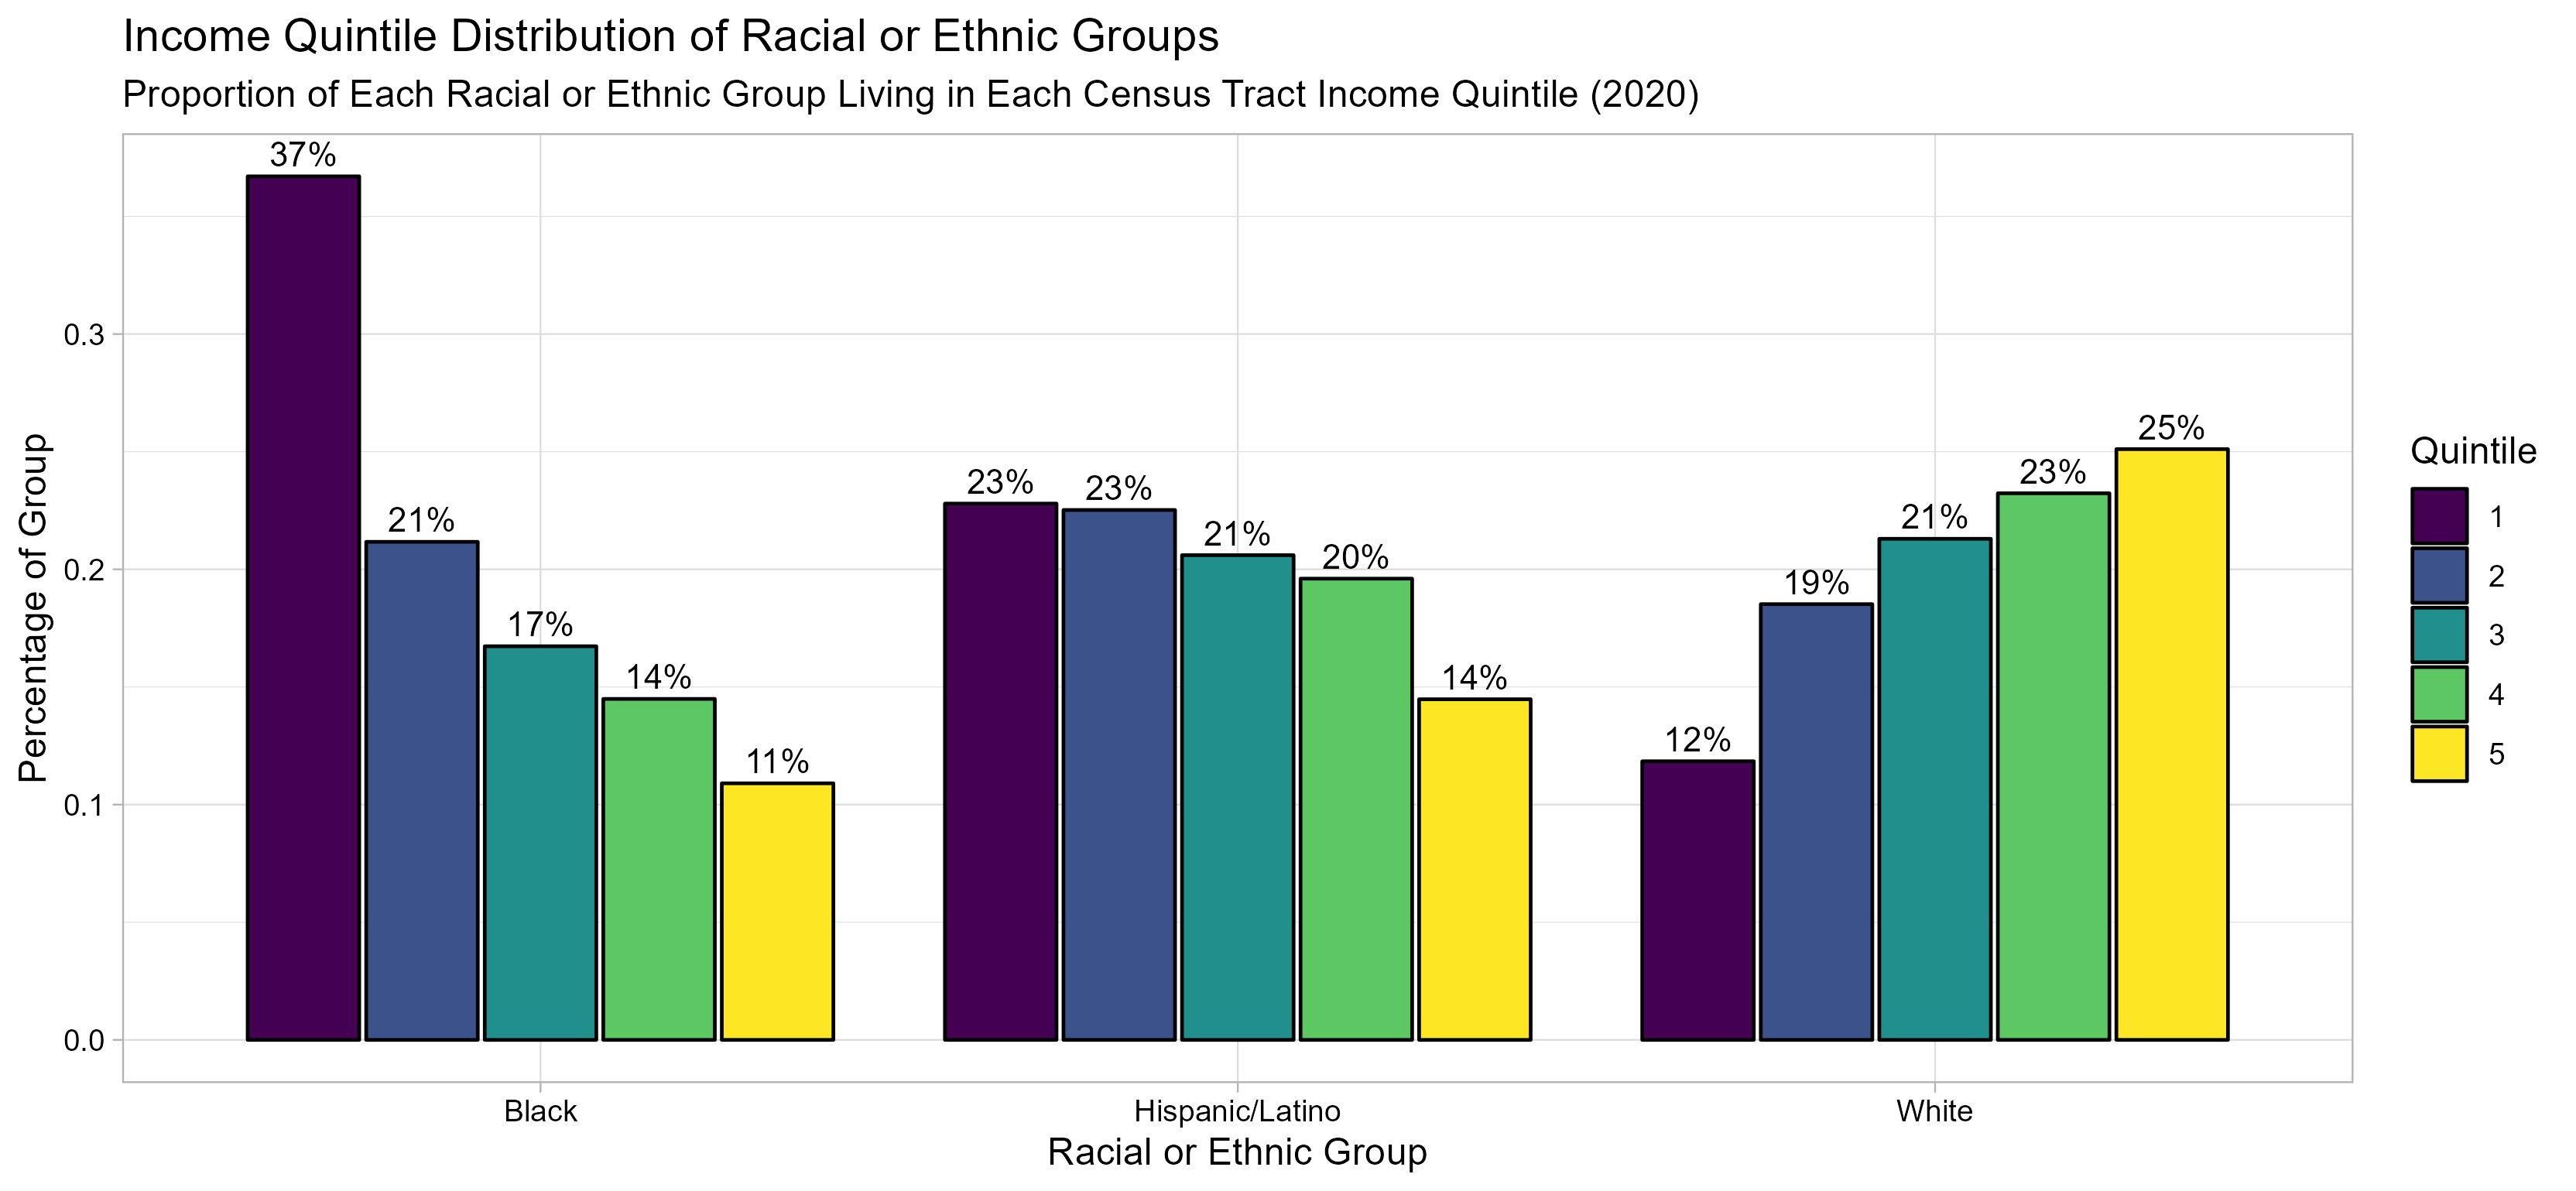
\includegraphics[width=\linewidth]{images/total_pop_quintiles_race}
  \captionsetup{justification=centering, singlelinecheck=false, margin=2cm}
  \caption{Race/Ethnicity Across Tract Income Quintiles}
  \label{fig:total_pop_quintiles_race}
\end{figure}

Analyses of the distribution of LUOF victims by race and income support similar conclusions to the analysis using majority-one-race in a census tract as a factor, with some exceptions. There is a relationship between the tract median household income quintiles and the proportion of each racial or ethnic group killed within each tract income quintile (\autoref{fig:inc_and_race_victim}). For example, 47.6 percent of black Americans who were killed by law enforcement were killed in the lowest income quintile of census tracts; just over 20 percent were killed in tracts in the second income quintile. There is the same relationship across all tracts where blacks were killed: the higher the income quintile, the lower the proportion. Only 6.7 percent of blacks were killed in the lowest-income census tracts. Latinos/Hispanics showed a similar trend, with 32.2 percent of all Latinos being killed in the lowest income quintile census tracts and only 9.9 percent killed in the highest income quintile. Interestingly, the largest proportion of whites were not killed in the lowest-income quintile tracts but in the second-lowest-income quintile tracts.

\begin{figure}[H]
  \centering
  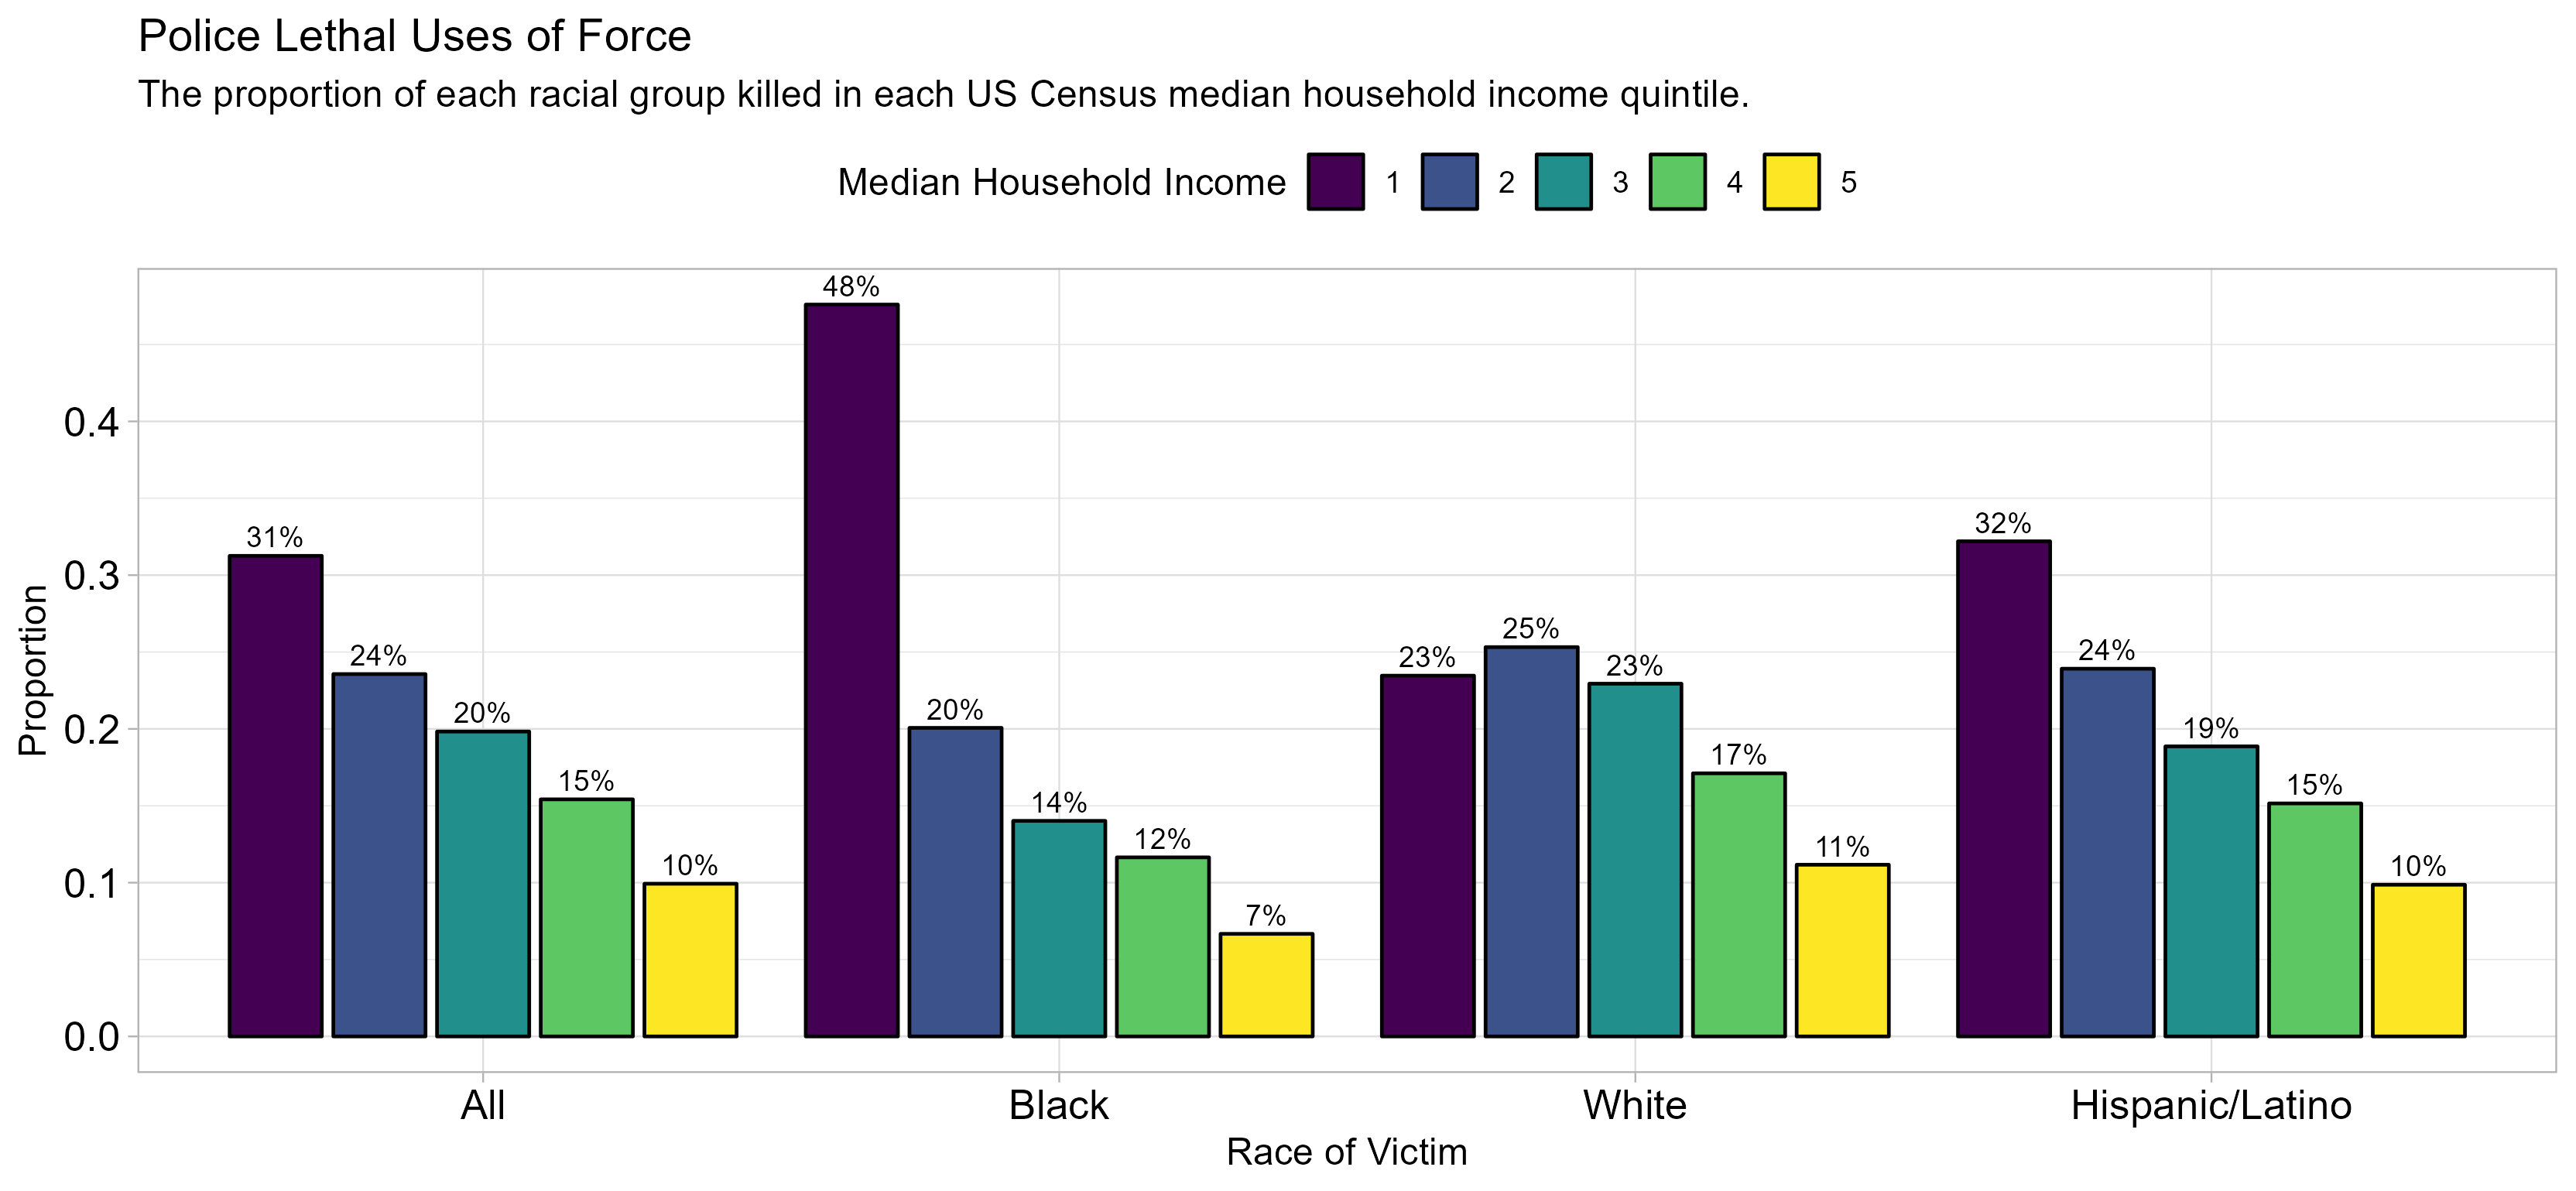
\includegraphics[width=\linewidth]{images/inc_and_race_victim}
  \captionsetup{justification=centering, singlelinecheck=false, margin=2cm}
  \caption{Proportion of Each Race Killed in Each Income Quintile}
  \label{fig:inc_and_race_victim}
\end{figure}


Comparisons between the population distribution of each race in income quintiles and the distribution of LUOFs across income quintiles reveal an interesting disparity. For example, while 36.7 percent of blacks live in the lowest income quintile, 47.6 percent of blacks killed by law enforcement were killed in tracts in the lowest income quintile. The same disproportionate trend holds for every other race/ethnicity: 22.8 percent of Latinos live in the lowest income quintile tracts, but 32.2 percent of Latinos killed by law enforcement were killed in the lowest income quintile tracts, and 11.8 percent of whites live in tracts in the lowest income quintile, but 23.5 percent of whites killed by law enforcement were killed in the lowest income quintile tracts.

\autoref{fig:inc_and_race_victim_shape_bar} places these data side-by-side, providing a visualization of how the two distributions in \autoref{fig:total_pop_quintiles_race} and \autoref{fig:inc_and_race_victim}. If the data bars were exactly the same across each row, it would indicate that the distribution of the racial group population across income quintiles is the same as the distribution of LUOFs within each group. But this is not the case. Moreover, Blacks and Latinos experience the greatest share of LUOFs in the lowest income quintile, greater than their incidence in that quintile. As noted earlier, there is an anomaly; slightly more whites— 25.3 percent—were killed in the second income quintile tracts than in the lowest income quintile—23.5 percent. Notwithstanding this anomaly, there is still a striking disparity between the proportion of whites living in the lowest-income tracts and the proportion of whites killed in those tracts.

\begin{figure}[H]
  \centering
  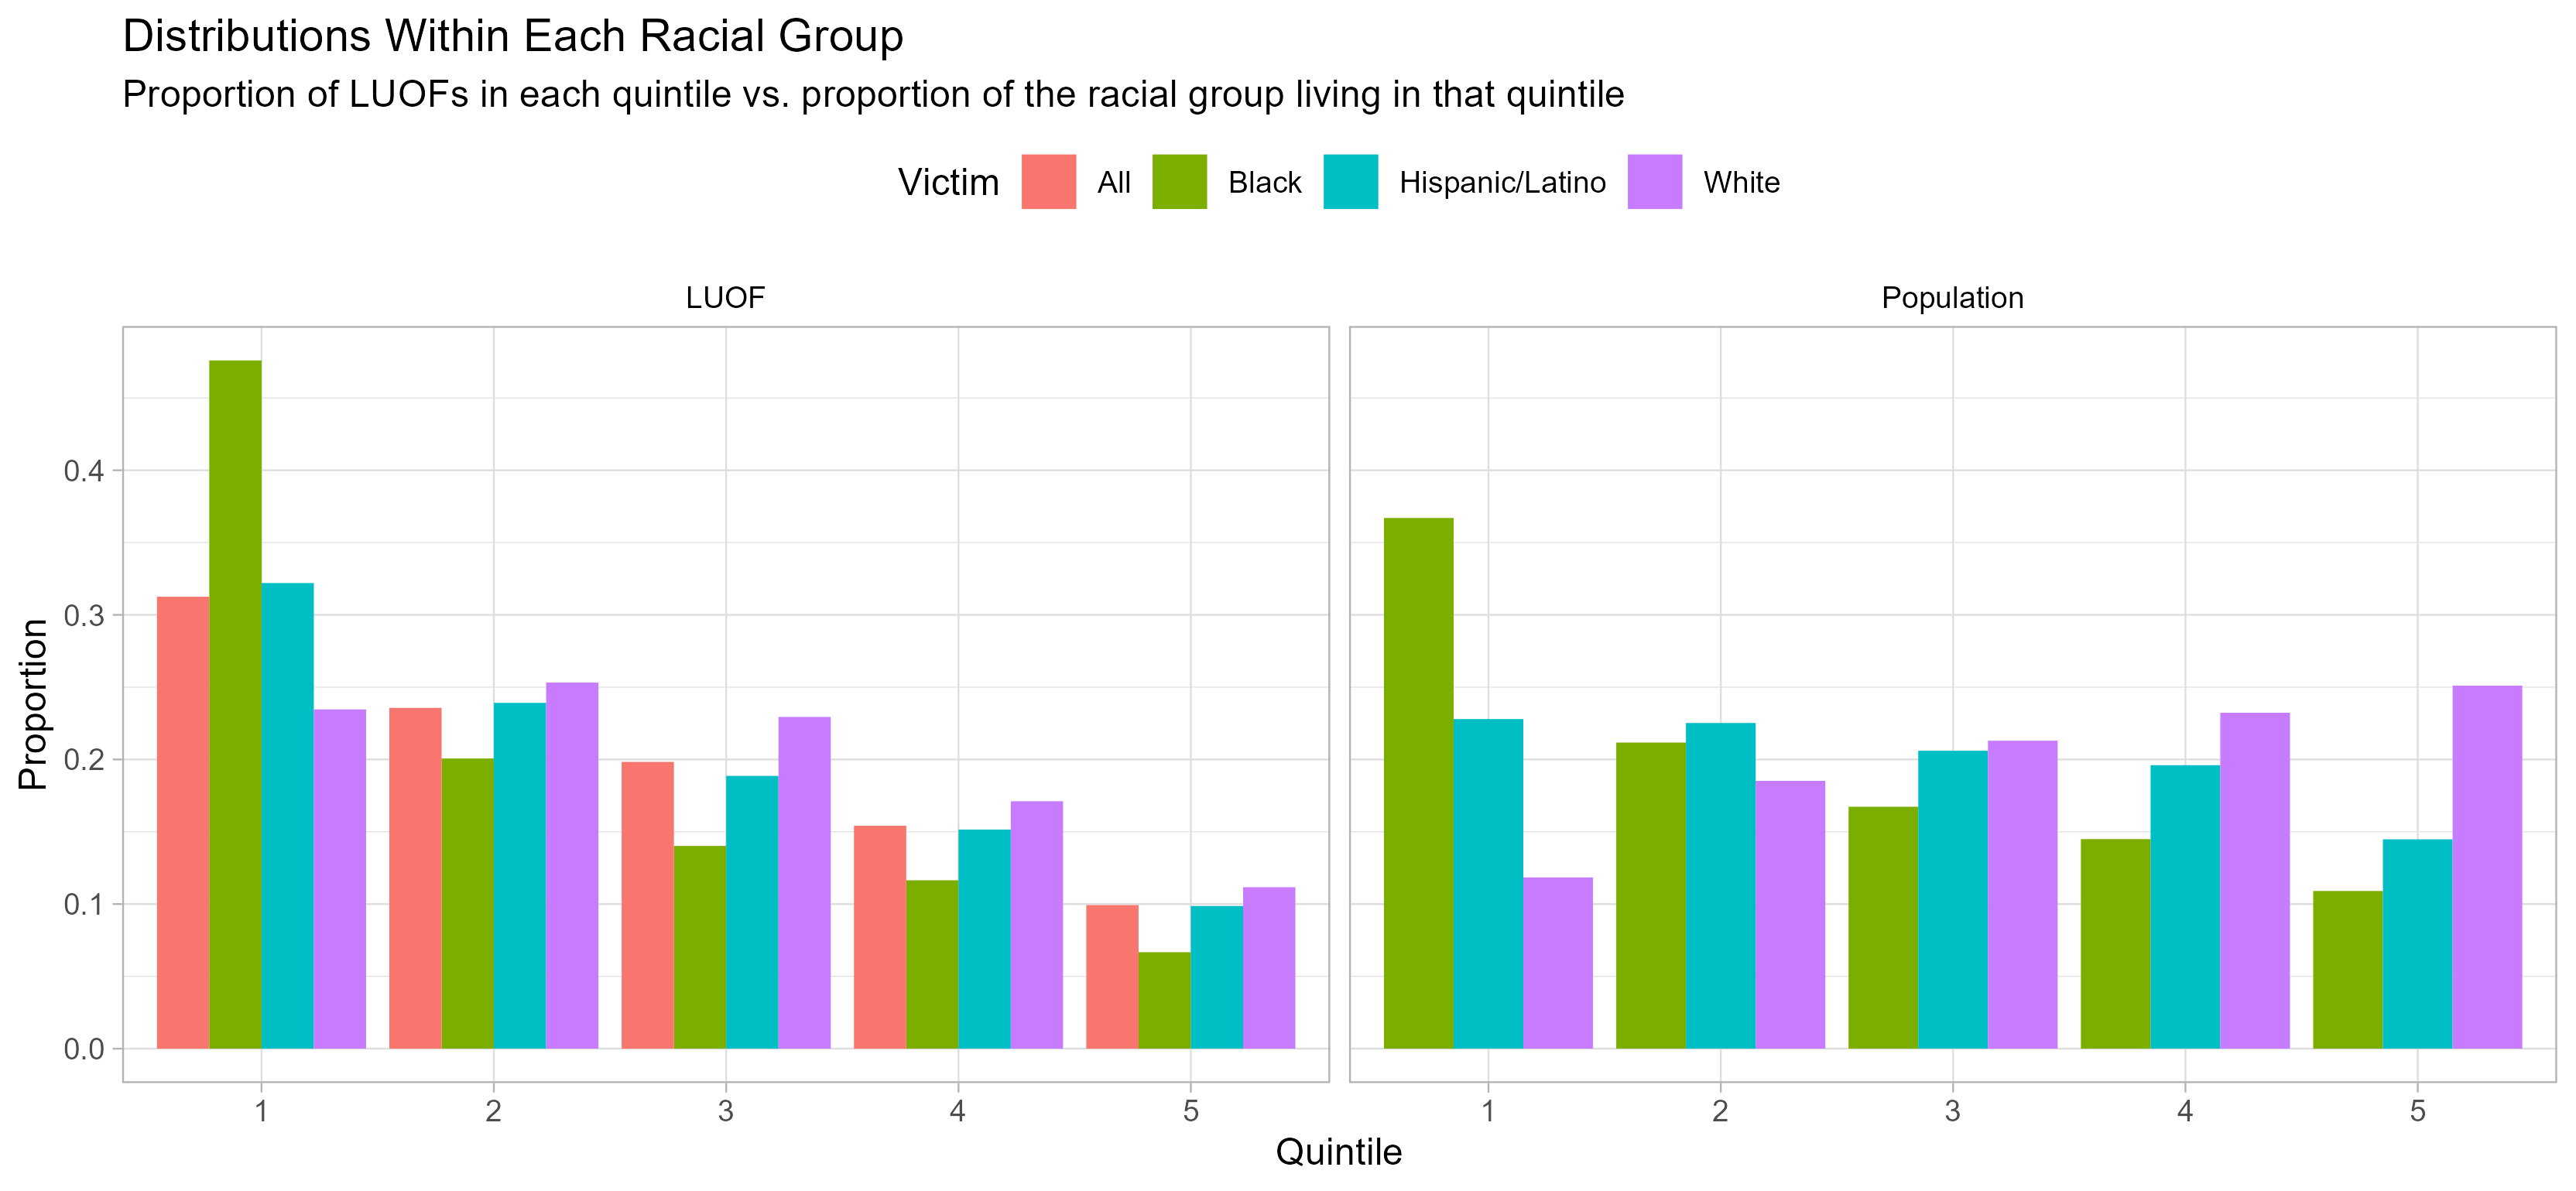
\includegraphics[width=\linewidth]{images/inc_and_race_victim_shape_bar}
  \captionsetup{justification=centering, singlelinecheck=false, margin=2cm}
  \caption{Proportion of Race Living in Income Quintile X vs. Proportion of Race Killed in Income Quintile X}
  \label{fig:inc_and_race_victim_shape_bar}
\end{figure}

\section{DISCUSSION}

In addition to racial disparities between racial and ethnic groups, the data show a clear relationship between median household income in census tracts where lethal uses of force (LUOFs) occurred. Census tracts in the lowest income quintile experienced a rate of LUOFs 4.3 times greater than tracts in the highest income quintile. Although it would be a stretch to infer causality based strictly on these observational findings, it does support some claims made by Cedric Johnson and the sociologist Loïc Wacquant, that racial subordination needs to be understood in the context of economic relations and how those also contribute to the likelihood of a LUOF.

The reasons for this are twofold. Policing practices and the corresponding outcomes—i.e., whether a LUOF is likely to occur, are influenced by both space (both the racial composition and the class composition of the neighborhood) and the class position of the individuals. Police departments often craft their policies in a way that concentrates the presence of law enforcement in the most economically marginal neighborhoods. At the same time, these neighborhoods are also disproportionately black and Latino. As Soss and Weaver explain, this is also driven by “tough on crime” measures, responses to both real and imagined incidents of crime. That is to say that intensified policing is advanced by political entrepreneurs agitating for these policies, but that agitation is only effective in the context of some increase in criminal activity.

\subsection{Limitations and Future Research} \

The limitation of this study is that it relied solely on observational data that were not well-suited for causal inference. Though there is a strong association between economic factors, such as income, and the incidence of police killings, it is difficult to rule out other factors that could be producing the outcome instead. It is always possible that other non-economic factors (at least not economic in a strict sense) related to the police budget or municipal politics could be driving the incidence of police killings as much as or more than the economic deprivation of a neighborhood or region. It is also possible, though probably less likely, that the causal path is in reverse to what has been suggested in this paper, that the high LUOF rate is leading to lower neighborhood incomes and impoverishment.
% \clearpage
\section{APPENDIX}

\begin{figure}[H]
  \centering % width=\linewidth, height=\textheight
  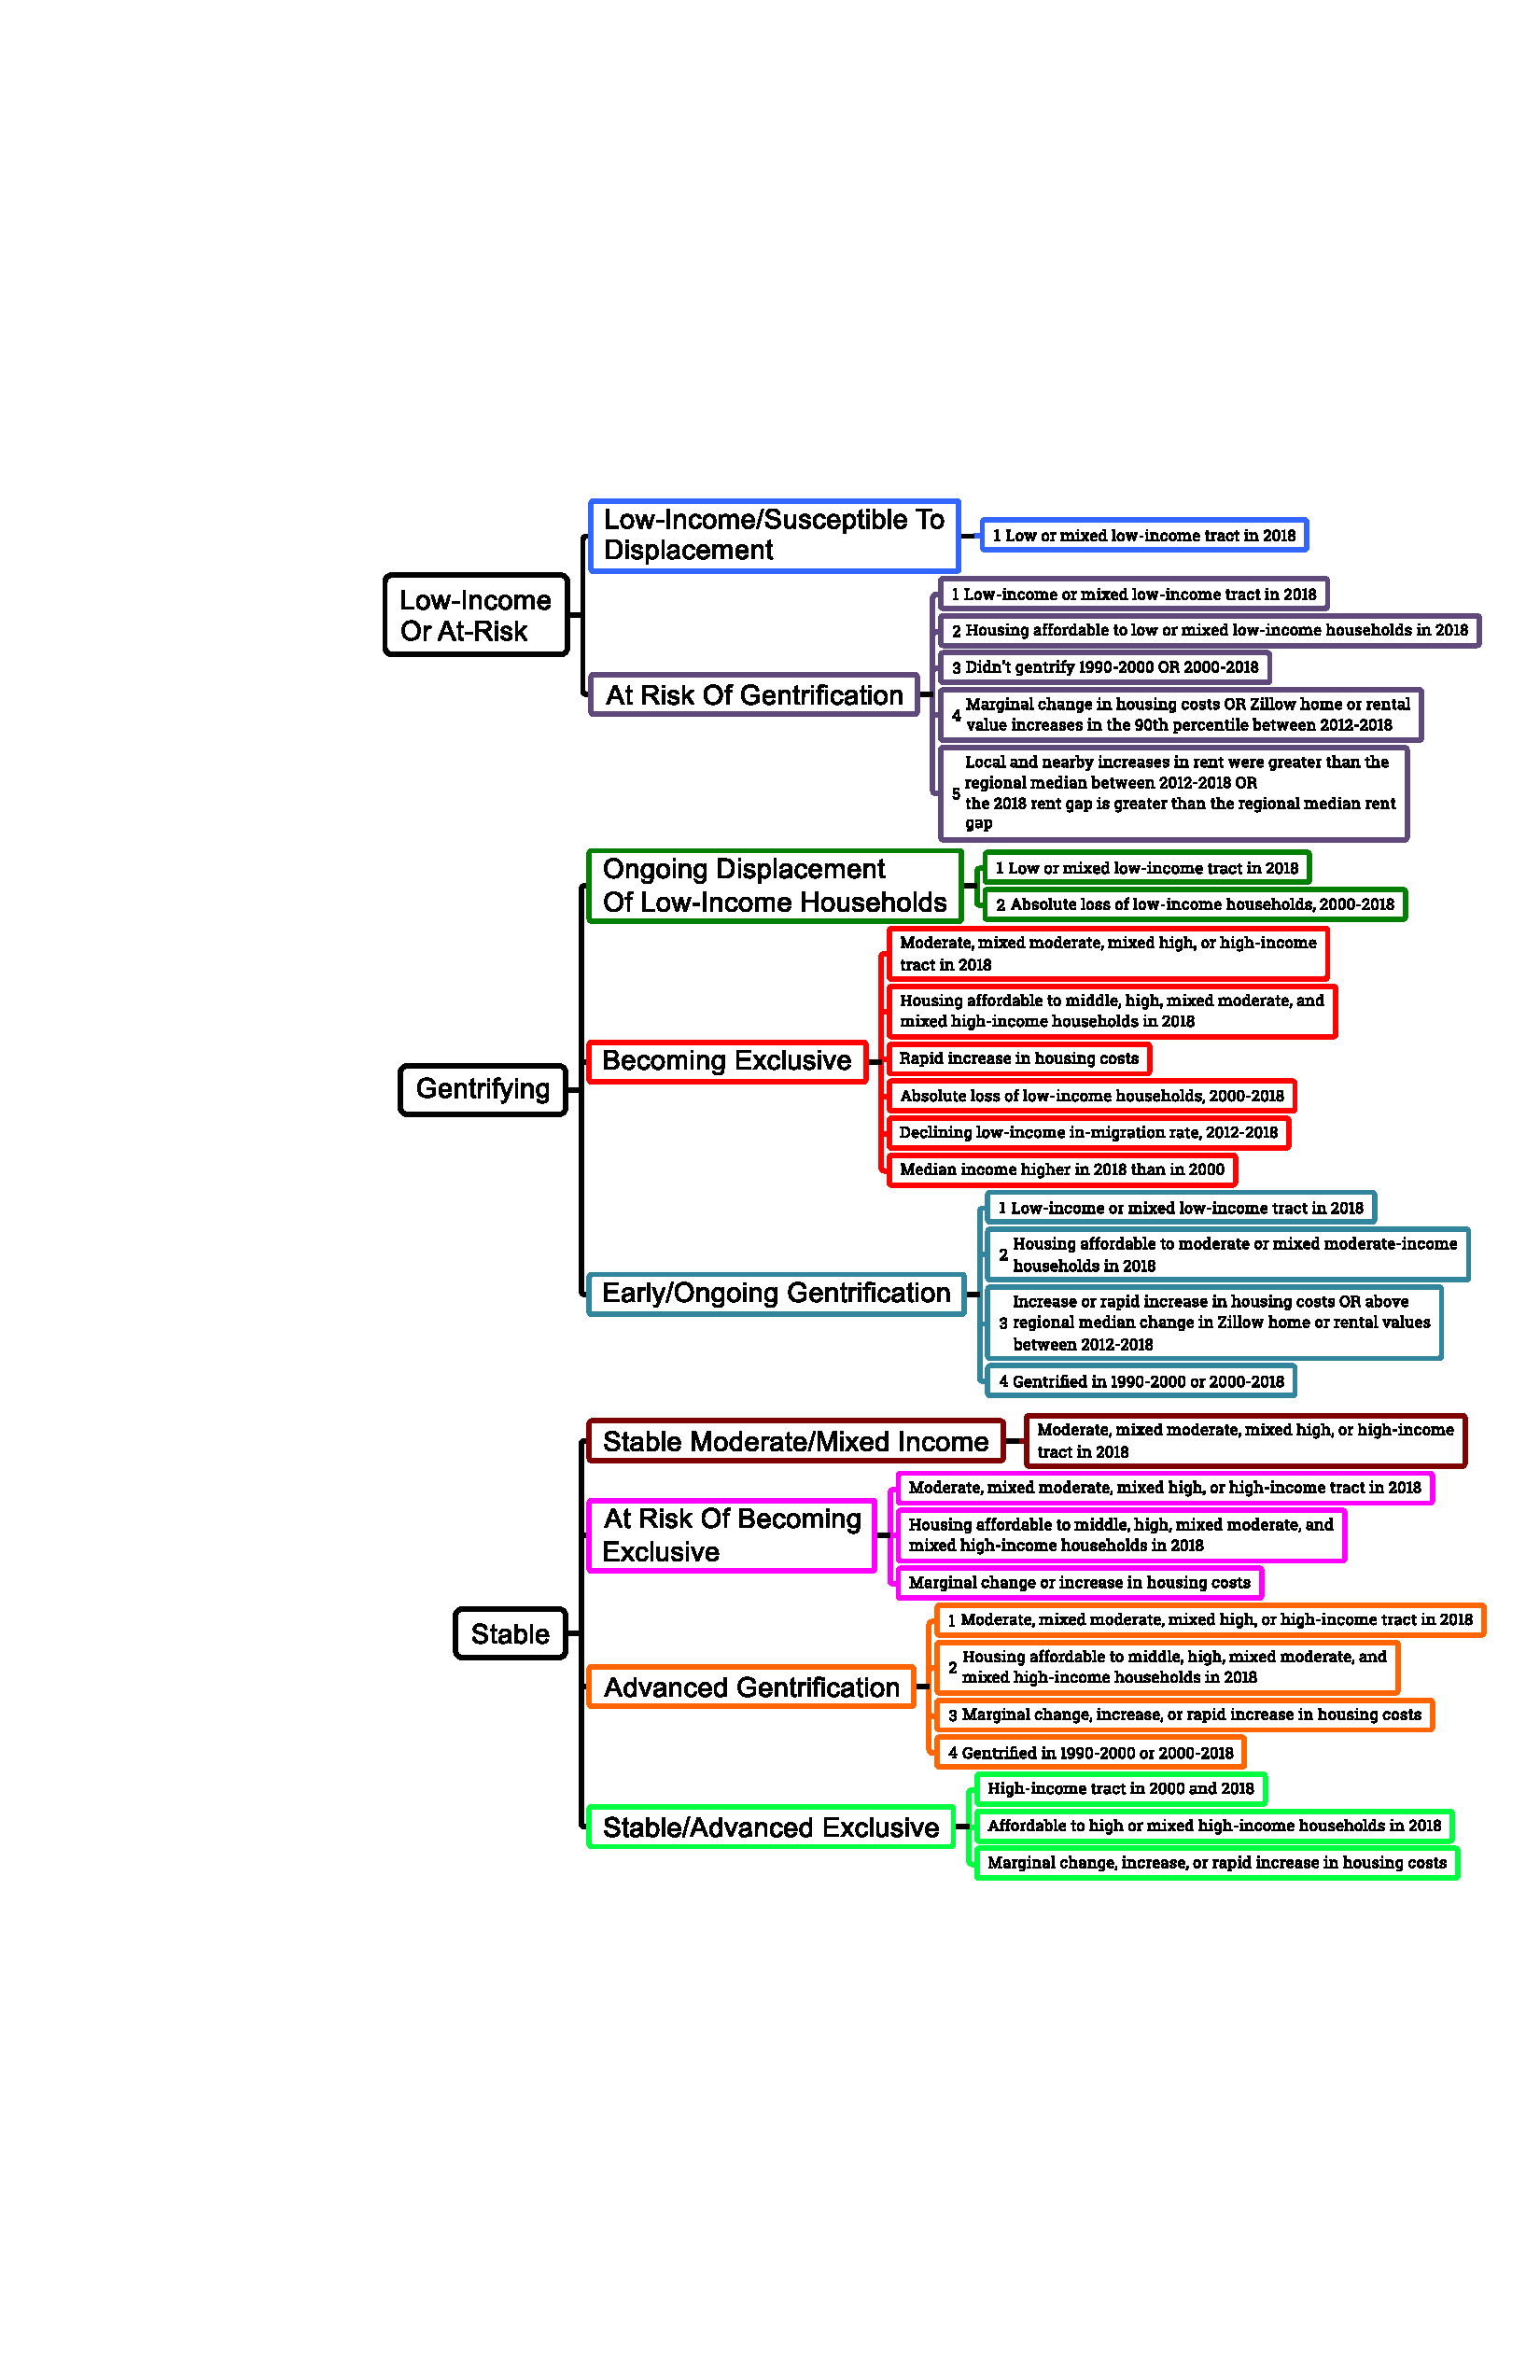
\includegraphics[width=\linewidth]{images/modified_typologies}
  \captionsetup{justification=centering, singlelinecheck=false, margin=2cm}
  \caption[Modified UDP Displacement Typologies]{Modified Urban Displacement Project (UDP) Typologies.}
  \label{fig:modified_typologies}
\end{figure}

\begin{figure}%[H]
  \centering % width=\linewidth, height=\textheight
  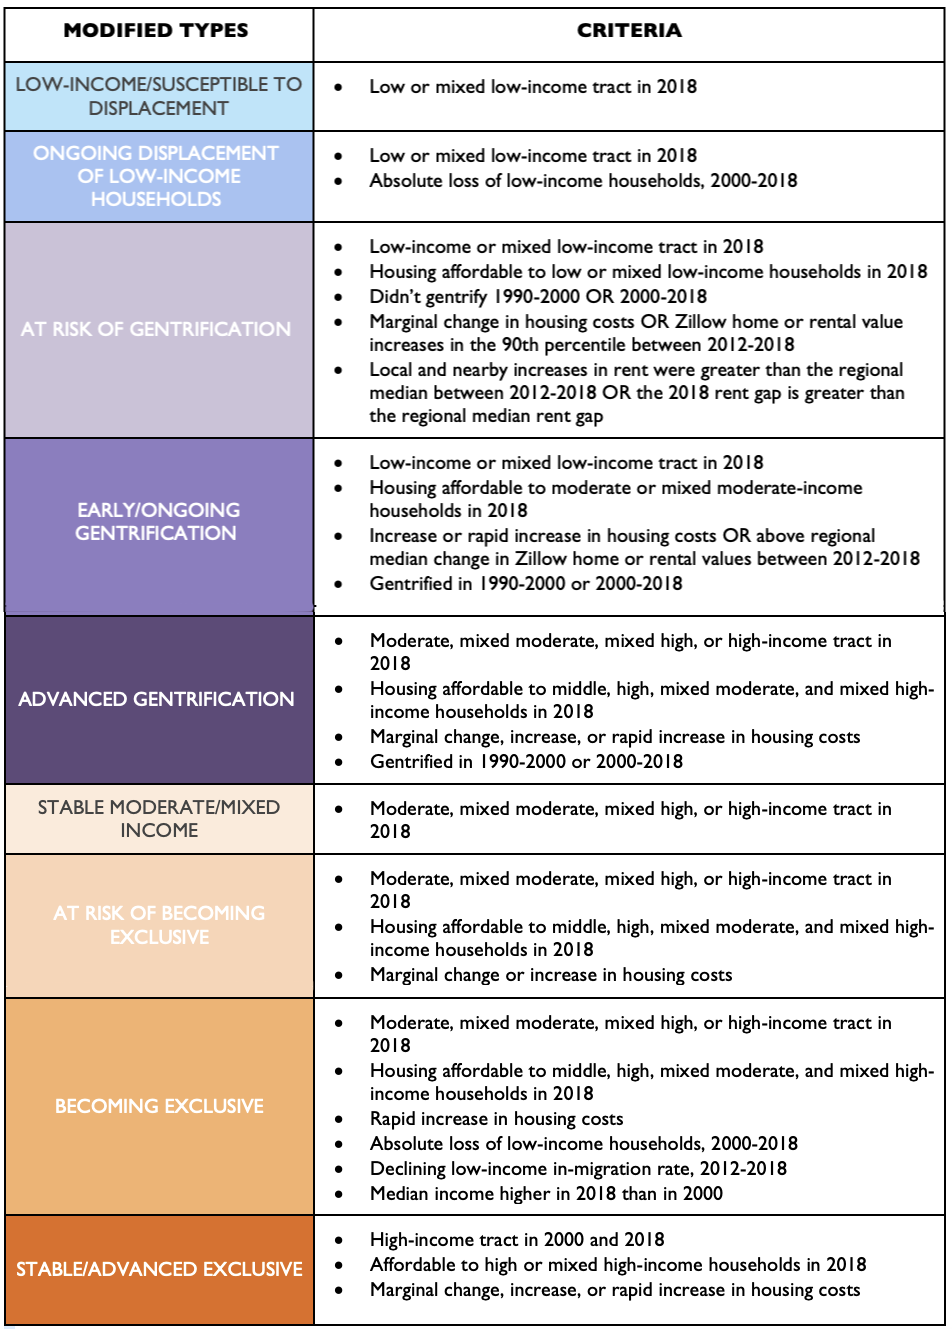
\includegraphics[height=0.95\textheight]{images/typology_sheet_2018}
  \captionsetup{justification=centering, singlelinecheck=false, margin=2cm}
  \caption[UDP Displacement Typologies]{Original Urban Displacement Project (UDP) Typologies.}
  \label{fig:original_udp}
\end{figure}

\clearpage
\sloppy


\titleformat{\section}{\fontsize{12}{14}\bfseries\centering}{\thesection}{0.5em}{}
% Line spacing
\setstretch{1.25}
\printbibliography[heading=bibintoc]

%\clearpage

%\paperwidth=\pdfpageheight
%\paperheight=\pdfpagewidth
%\pdfpageheight=\paperheight
%\pdfpagewidth=\paperwidth
%\headwidth=\textheight
%\begingroup 
%\vsize=\textwidth
%\hsize=\textheight

%\newpage
%\paperwidth=\pdfpageheight
%\paperheight=\pdfpagewidth
%\pdfpageheight=\paperheight
%\pdfpagewidth=\paperwidth
%\headwidth=\textwidth

\end{document}
